\graphicspath{{./figs/}}
\subsection{Ego}
\begin{frame}
    \frametitle{Current Progress}

    % Only shows the current section and its subsections, hides everything else
    \tableofcontents[currentsection,
                     subsectionstyle=show/shaded/hide,
                     sectionstyle=show/hide]

    % Explanation of options:
    % - currentsection: Highlights the current section
    % - subsectionstyle=show/show/hide: The current subsection and its siblings in the current section are shown
    % - sectionstyle=show/hide: Shows only the current section, hides other sections
\end{frame}


\begin{frame}
	\frametitle{Who Am I? — Basic Info}
	\begin{columns}
	\begin{column}{0.65\textwidth}
		\begin{itemize}
			\item Louis Ledoux, 29 yo, PhD arithmetic HW
			\item My website, a pointer to many things:
			\begin{itemize}
				\item papers
				\item CV
				\item projects
				\item this presentation's slides
			\end{itemize}
		\end{itemize}
	\end{column}
	\begin{column}{0.35\textwidth}
		\begin{figure}[H]
			\centering
			
\includegraphics[width=\textwidth]{QR-Mysite.png}
			\caption{https://bynaryman.github.io/}
			\label{fig:qr_website}
		\end{figure}
	\end{column}
	\end{columns}
\end{frame}

\begin{frame}
	\frametitle{Who Am I? — Research Interests}
	\begin{itemize}
		\item<1-> \textbf{Computer Architecture:}
		\begin{itemize}
			\item Floating-Point Units, Systolic Arrays, Matrix-Matrix Multiply (MMM) Units
			\item GPUs, FPGAs, workload-specific accelerators
		\end{itemize}
		\item<2-> \textbf{Computer Arithmetic:}
		\begin{itemize}
			\item Number Representations, Posit, IEEE 754 Standards
			\item FloPoCo, Application-Specific Circuits
			\item Kulisch Accumulator
		\end{itemize}
		\item<3-> \textbf{High Performance Computing:}
		\begin{itemize}
			\item BLAS, GEMMs, Heterogeneous Workloads
			\item Numerical Analysis, Supercomputing
		\end{itemize}
	\end{itemize}
\end{frame}

\begin{frame}
	\frametitle{Who Am I? — Education}
	\begin{itemize}
		\item<1-> \textbf{2013-2015} - Integrated Preparatory Class (CUPGE) - \textit{Rennes}
		\item<2-> \textbf{2015-2018} - ESIR (\'Ecole Supérieure d'Ing\'enieurs de \textit{Rennes})
		\begin{itemize}
			\item Engineer + Master's Degree, specializing in Computer Science.
			\item Last year coopt student at b<>com made me go to hardware
		\end{itemize}
		\item<3-> \textbf{2018-2024} - UPC (Universitat Politècnica de Catalunya) - \textit{Barcelona}
		\begin{itemize}
			\item Also Barcelona Supercomputing Center (BSC) / Marenostrum4/5
			\item Thesis: \textit{``Floating-Point Arithmetic Paradigms for High-Performance Computing: Software Algorithms and Hardware Designs''}
		\end{itemize}
		\item<4-> \textbf{2025-2027} - Coming Soon: Postdoc at INSA - \textit{Lyon}
		\begin{itemize}
			\item with Florent de Dinechin on MLIR-FloPoCo
		\end{itemize}
	\end{itemize}
\end{frame}

\begin{frame}
	\frametitle{Who Am I? — Hobbies}
	\begin{itemize}
		\item<1-> \textbf{Mixing science and art}
		\begin{itemize}
			\item Crafting weird instruments (FDD, HDD, scanner)
			\item Modular Synthesis (Eurorack)
			\item Visualing birth of chips
			\item Rendering chips polygons
			\item Hacking a bit of everything
			\item ...
		\end{itemize}
		\item<2-> \textbf{Time for a showcase}
		\begin{itemize}
			\item but let's talk about it afterwards :)
		\end{itemize}
	\end{itemize}
\end{frame}

\begin{frame}
	\frametitle{Render Systolic Array}
	\begin{figure}[H]
		\centering
		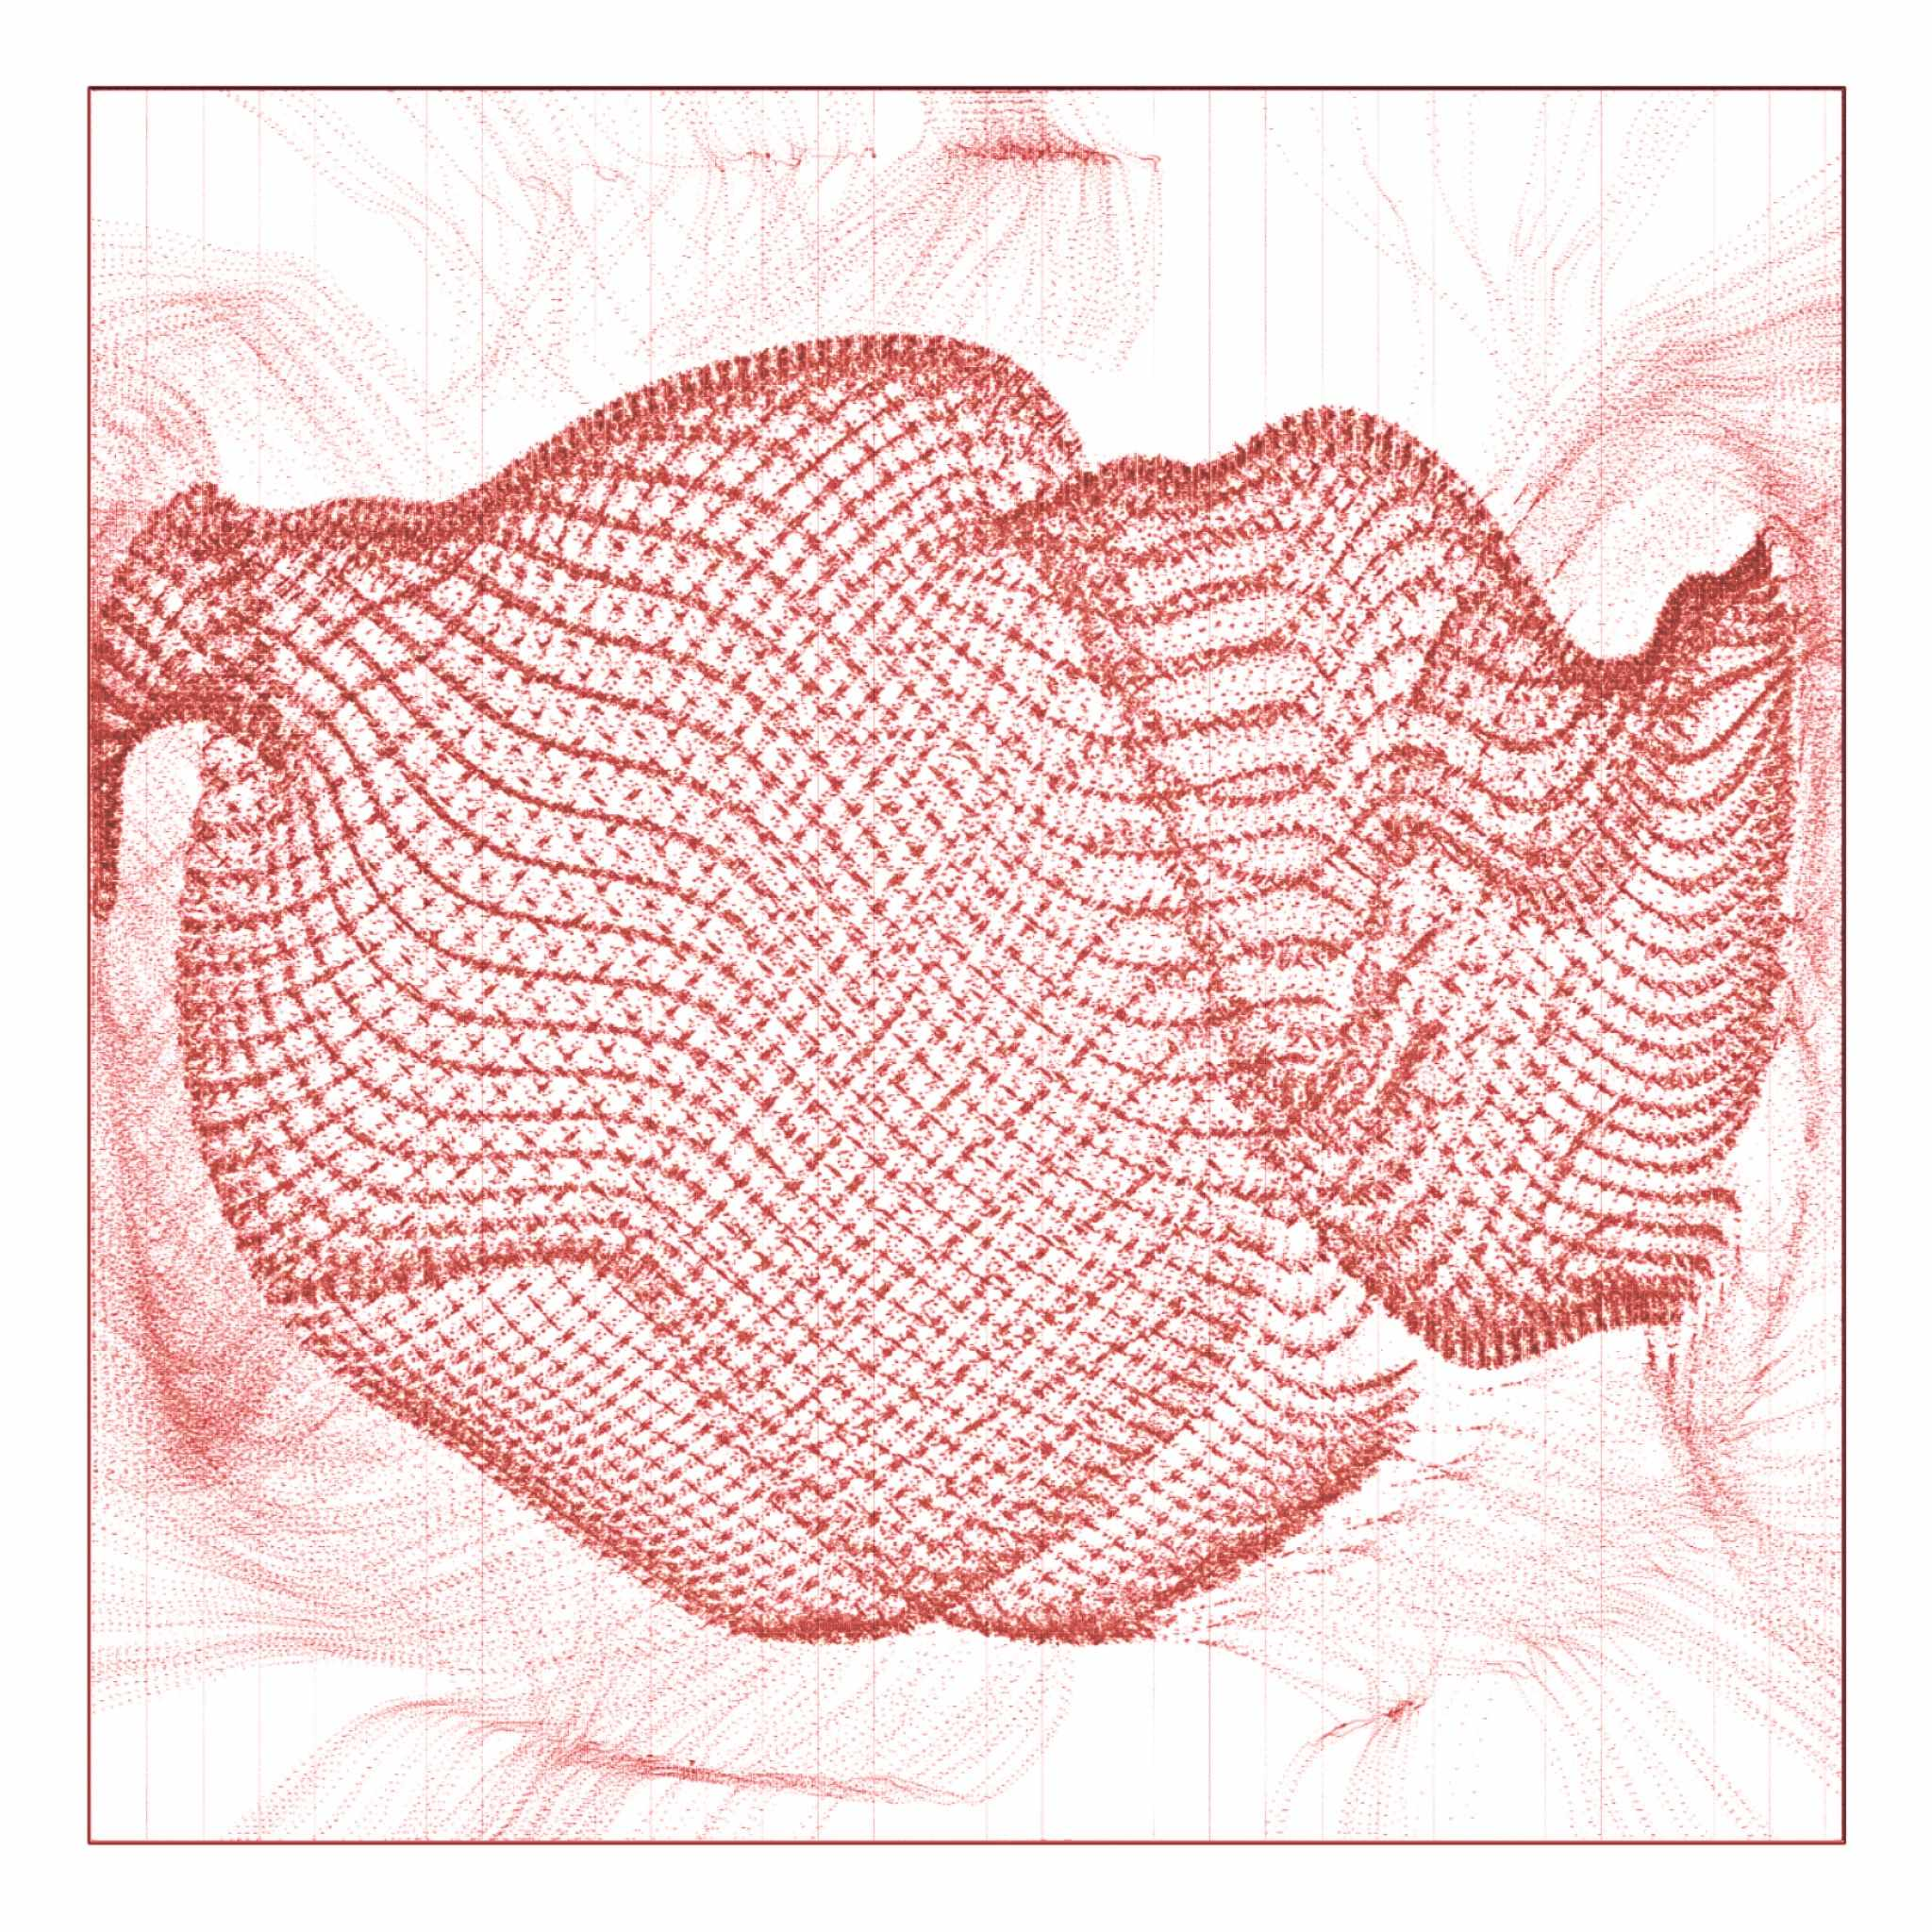
\includegraphics[width=0.5\textwidth]{4096PE.jpg}
		\caption{Edge detection iteration 256 neterov.}
		\label{fig:4096PE}
	\end{figure}
\end{frame}

\begin{frame}
	\frametitle{Systolic Array GDS Raytracing + artistic blur lens}
	\begin{figure}[H]
		\centering
		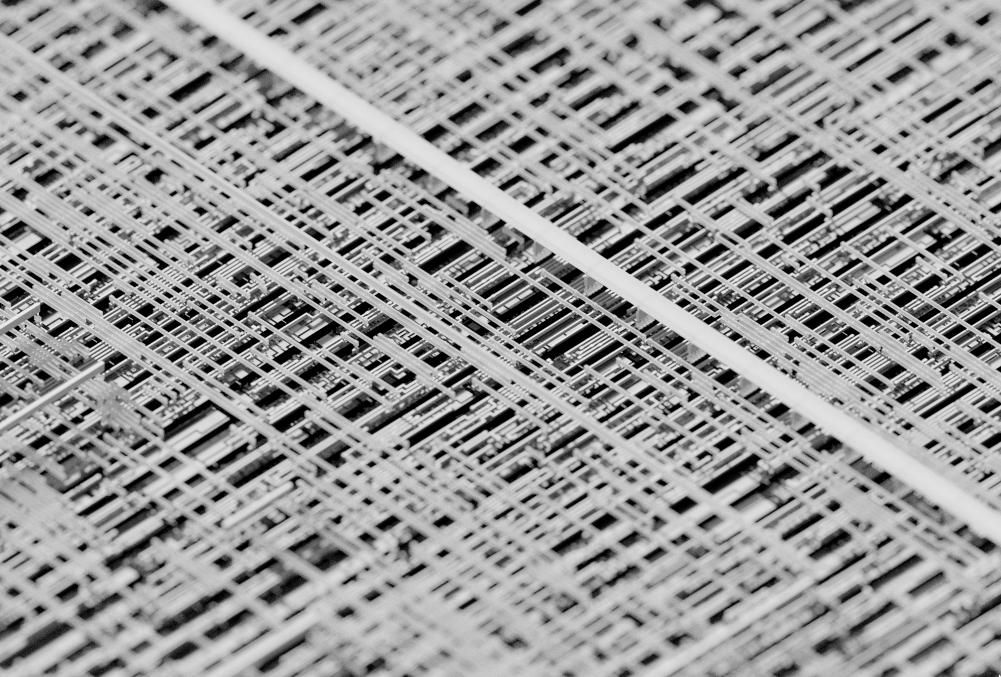
\includegraphics[width=0.8\textwidth]{teras.png}
		\caption{Raytracing W\&B and blur.}
		\label{fig:teras_raytracing}
	\end{figure}
\end{frame}

\begin{frame}
\frametitle{Systolic Array Tapeout}
\begin{figure}[H]
	\centering
	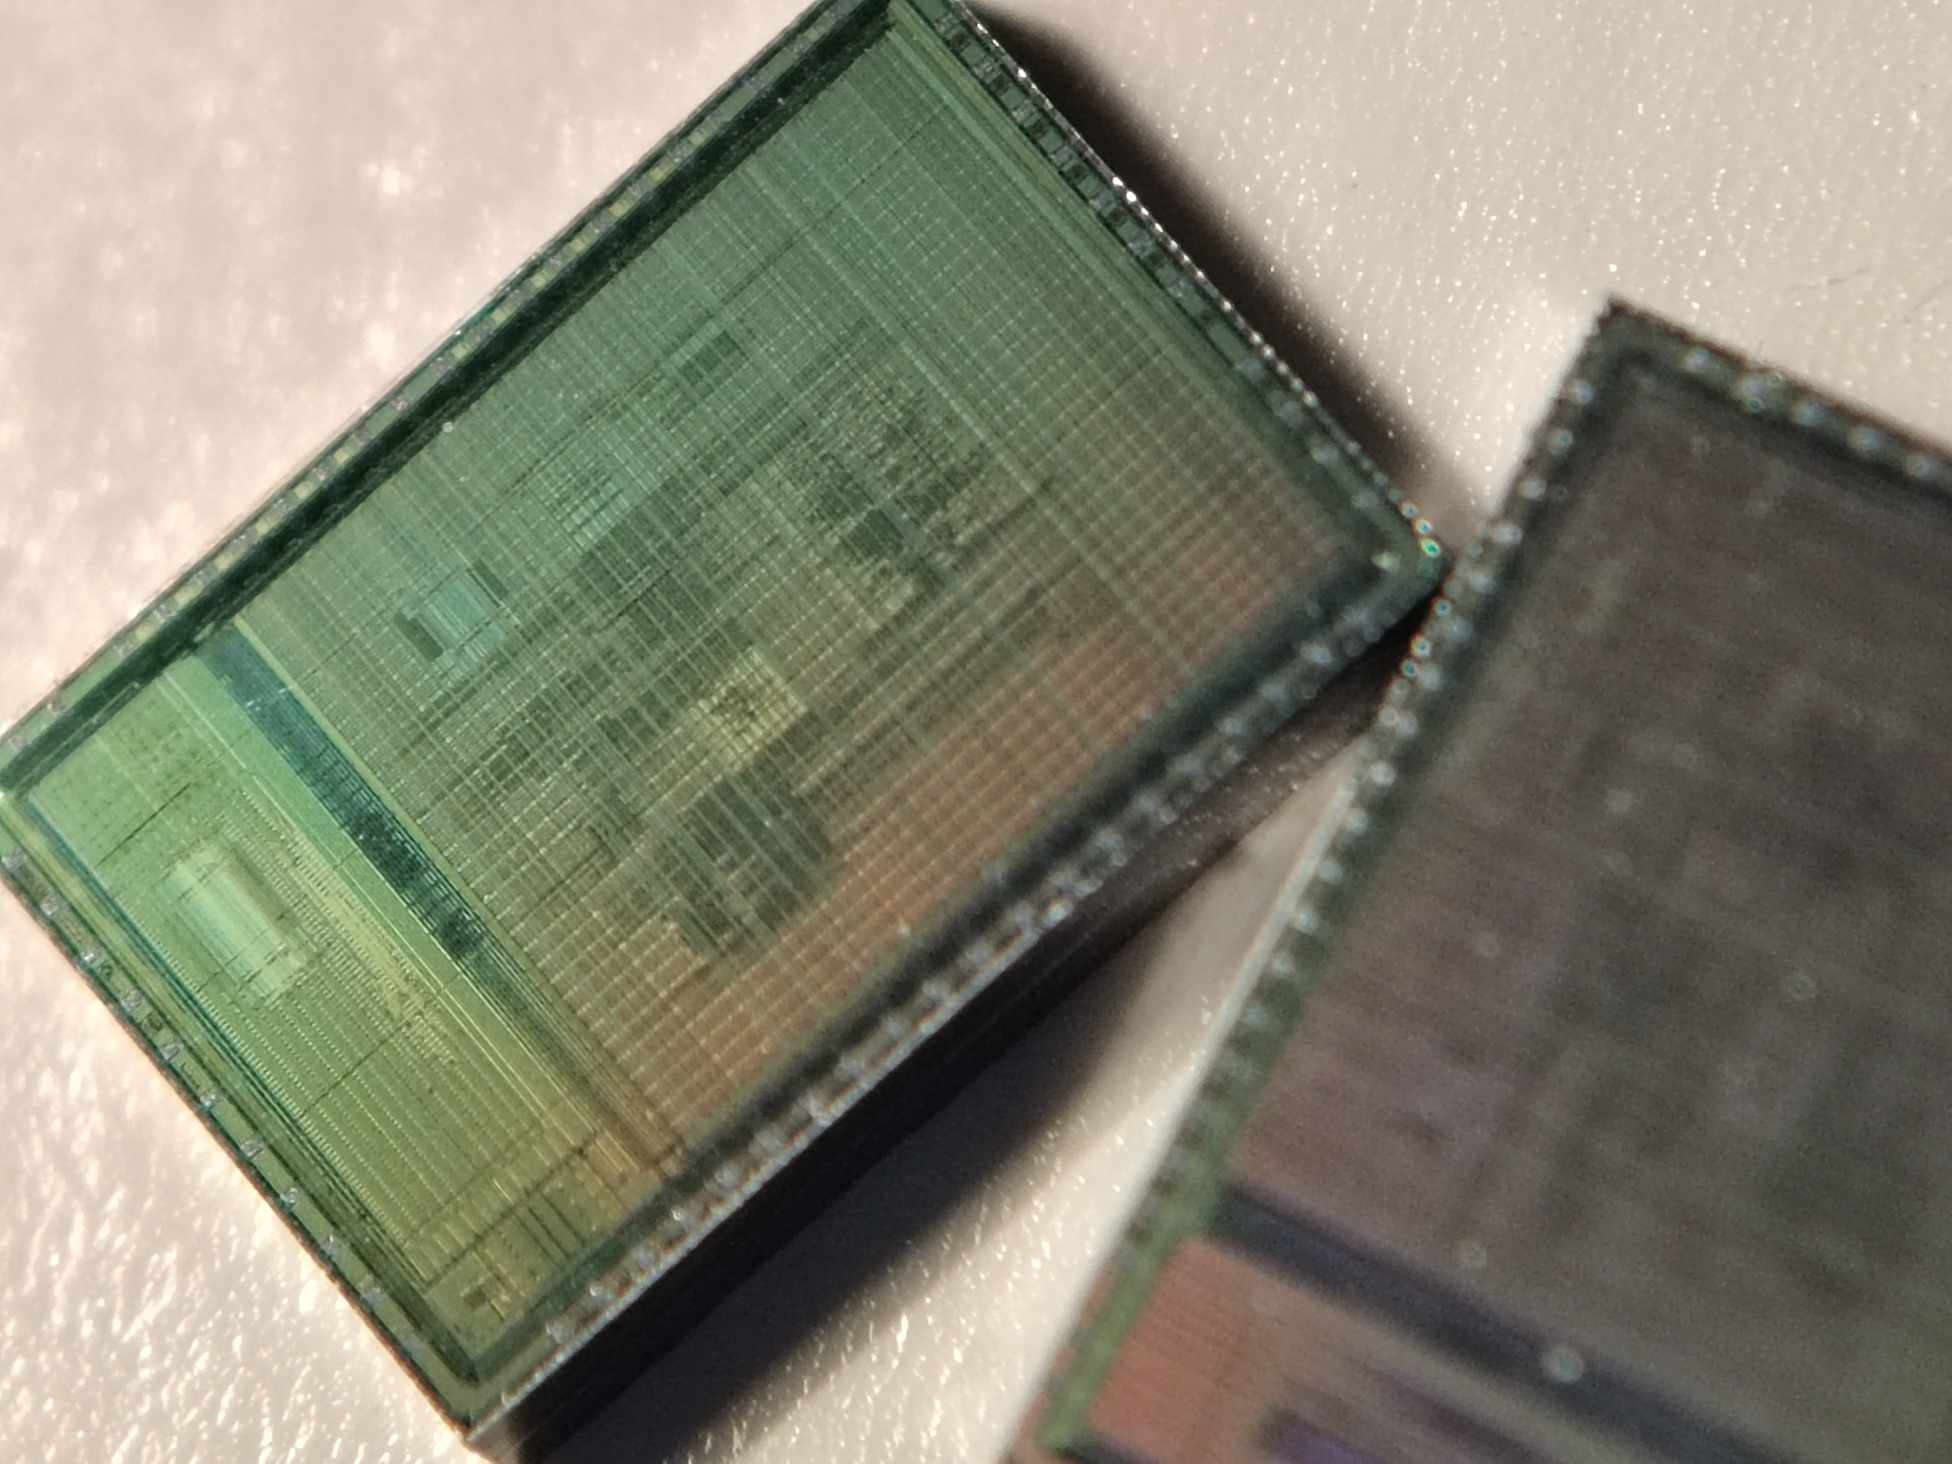
\includegraphics[width=0.7\textwidth]{tapeout_pic.jpg}
	\caption{Photo taken with a lens and a smartphone.}
\end{figure}
\end{frame}

\begin{frame}
\frametitle{303 Synthesizer reproduction}
\begin{figure}[H]
	\centering
	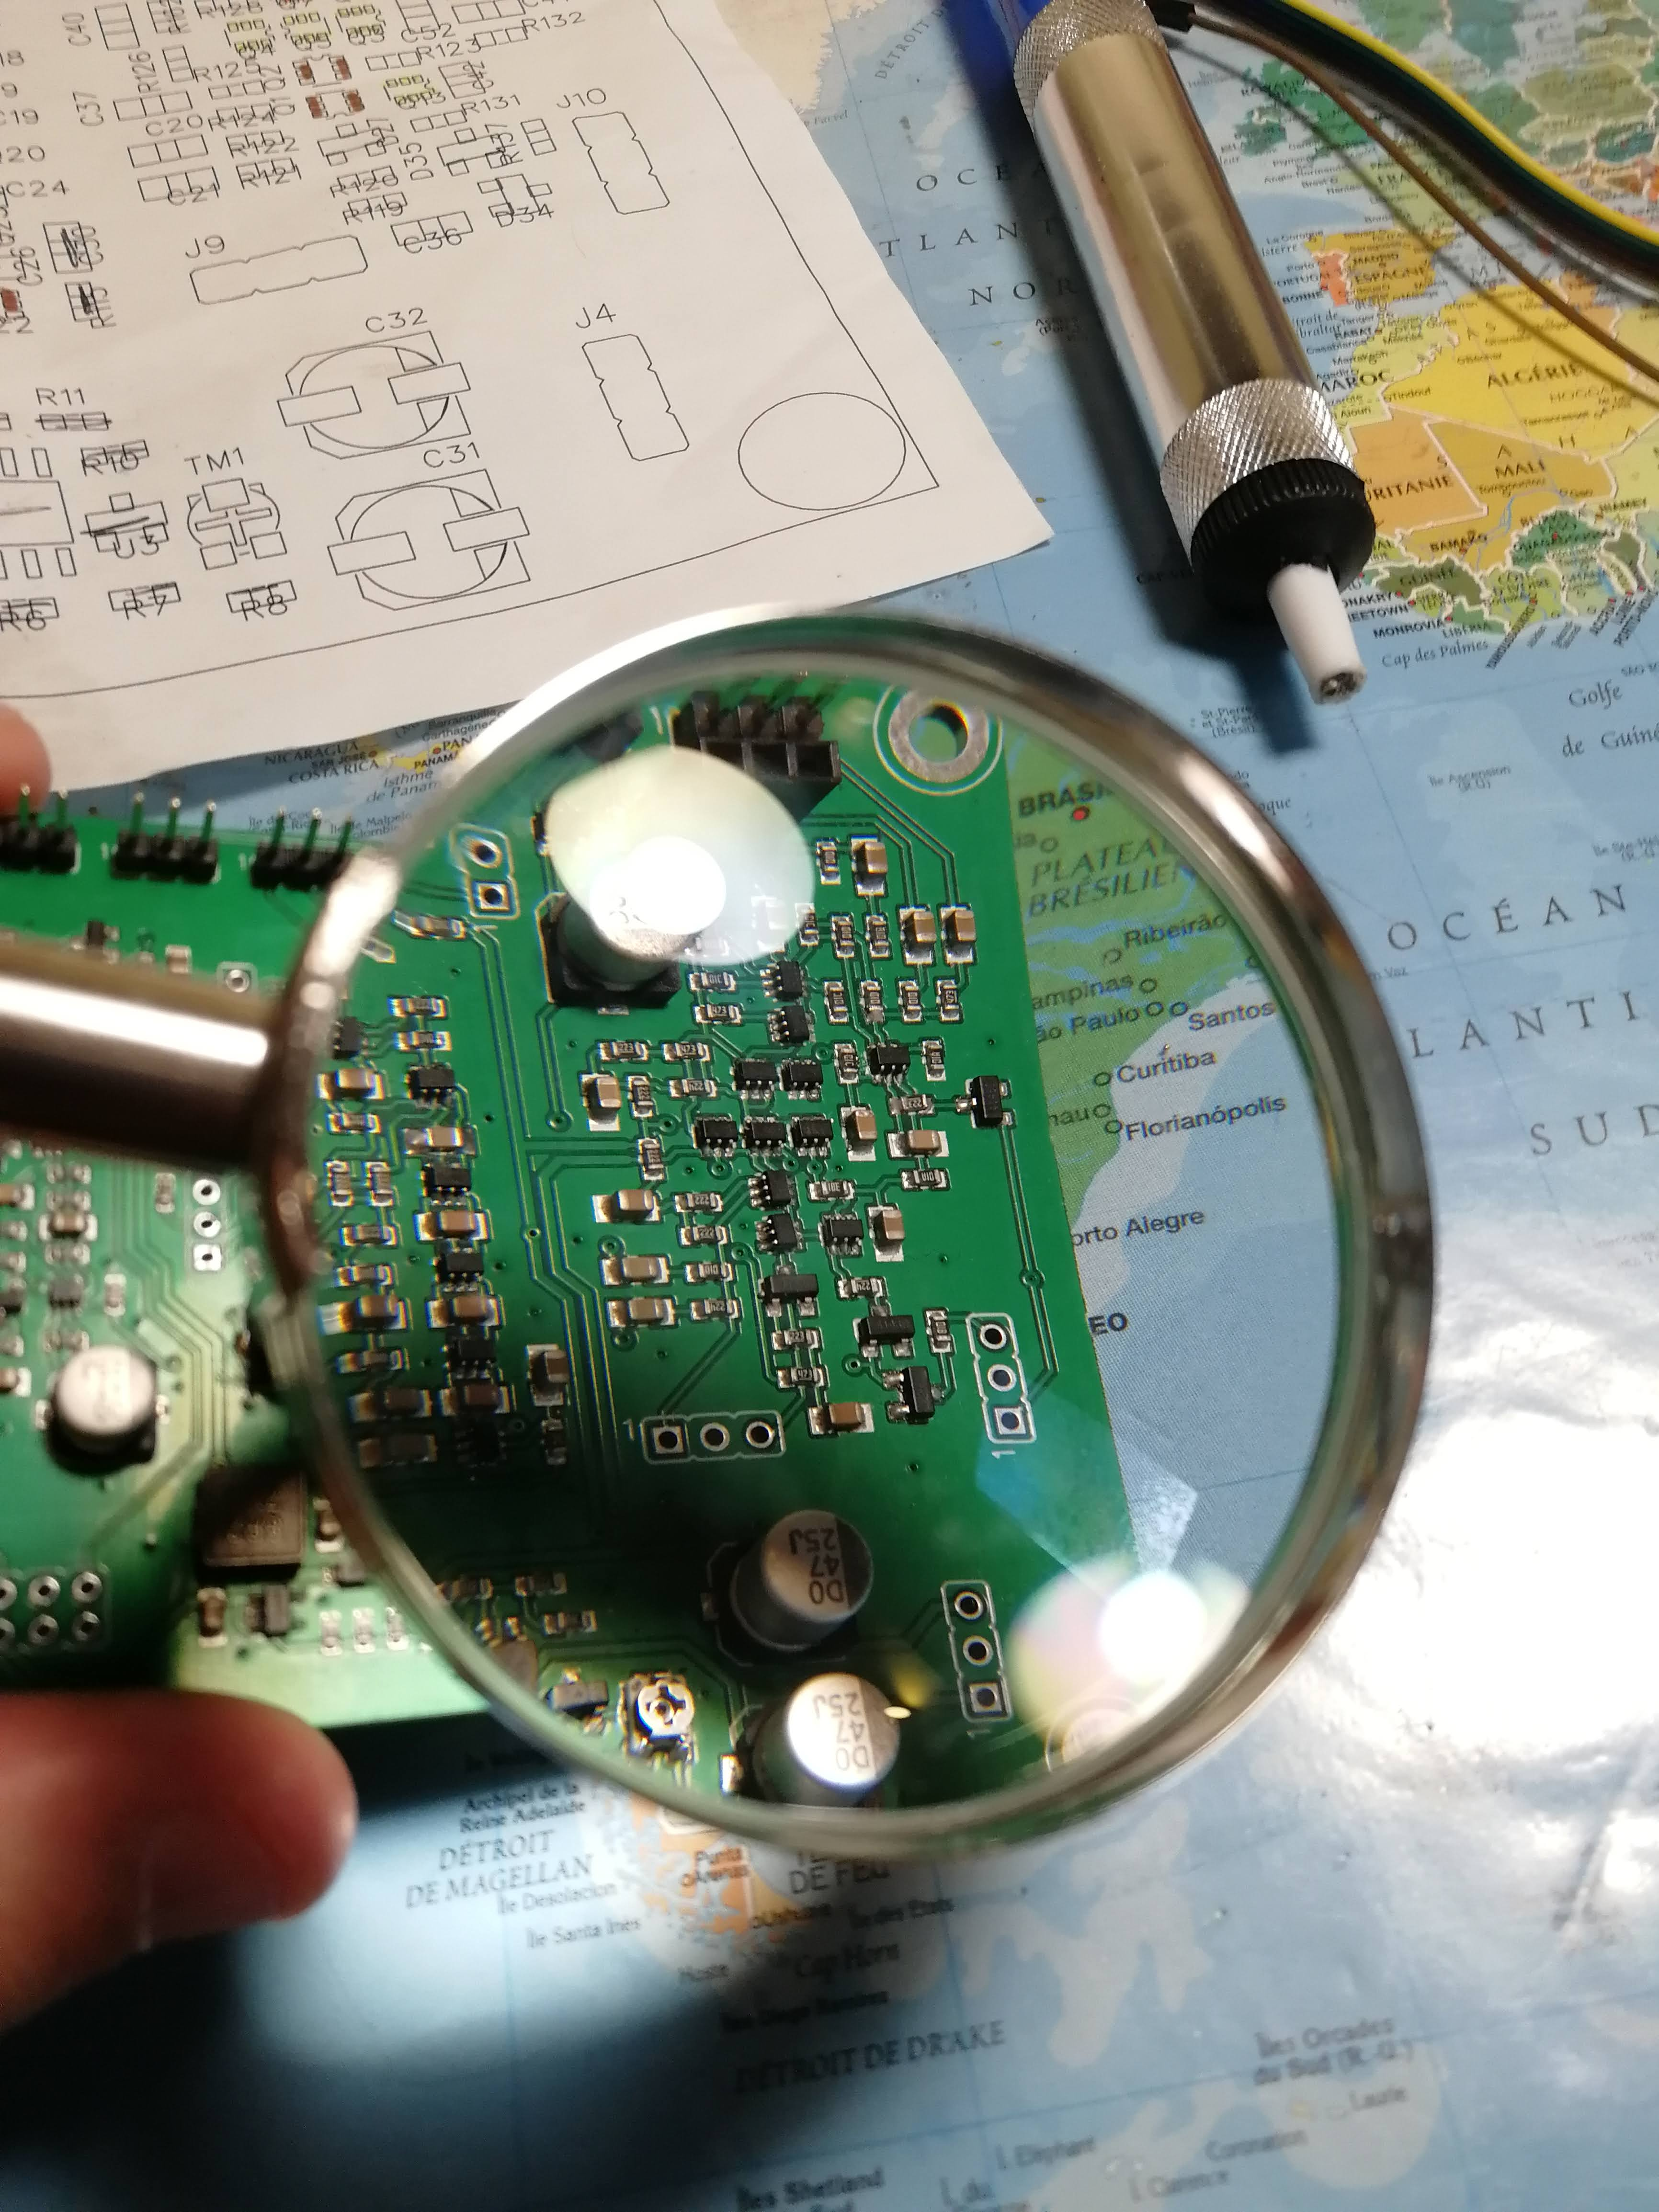
\includegraphics[width=0.4\textwidth]{analo_303.jpg}
	\caption{Proud of my weldings}
\end{figure}
\end{frame}

\begin{frame}
	\frametitle{Like steve jobs, my home lab :)}
\begin{columns}
\begin{column}{0.35\textwidth}
	\begin{figure}[H]
		\centering
		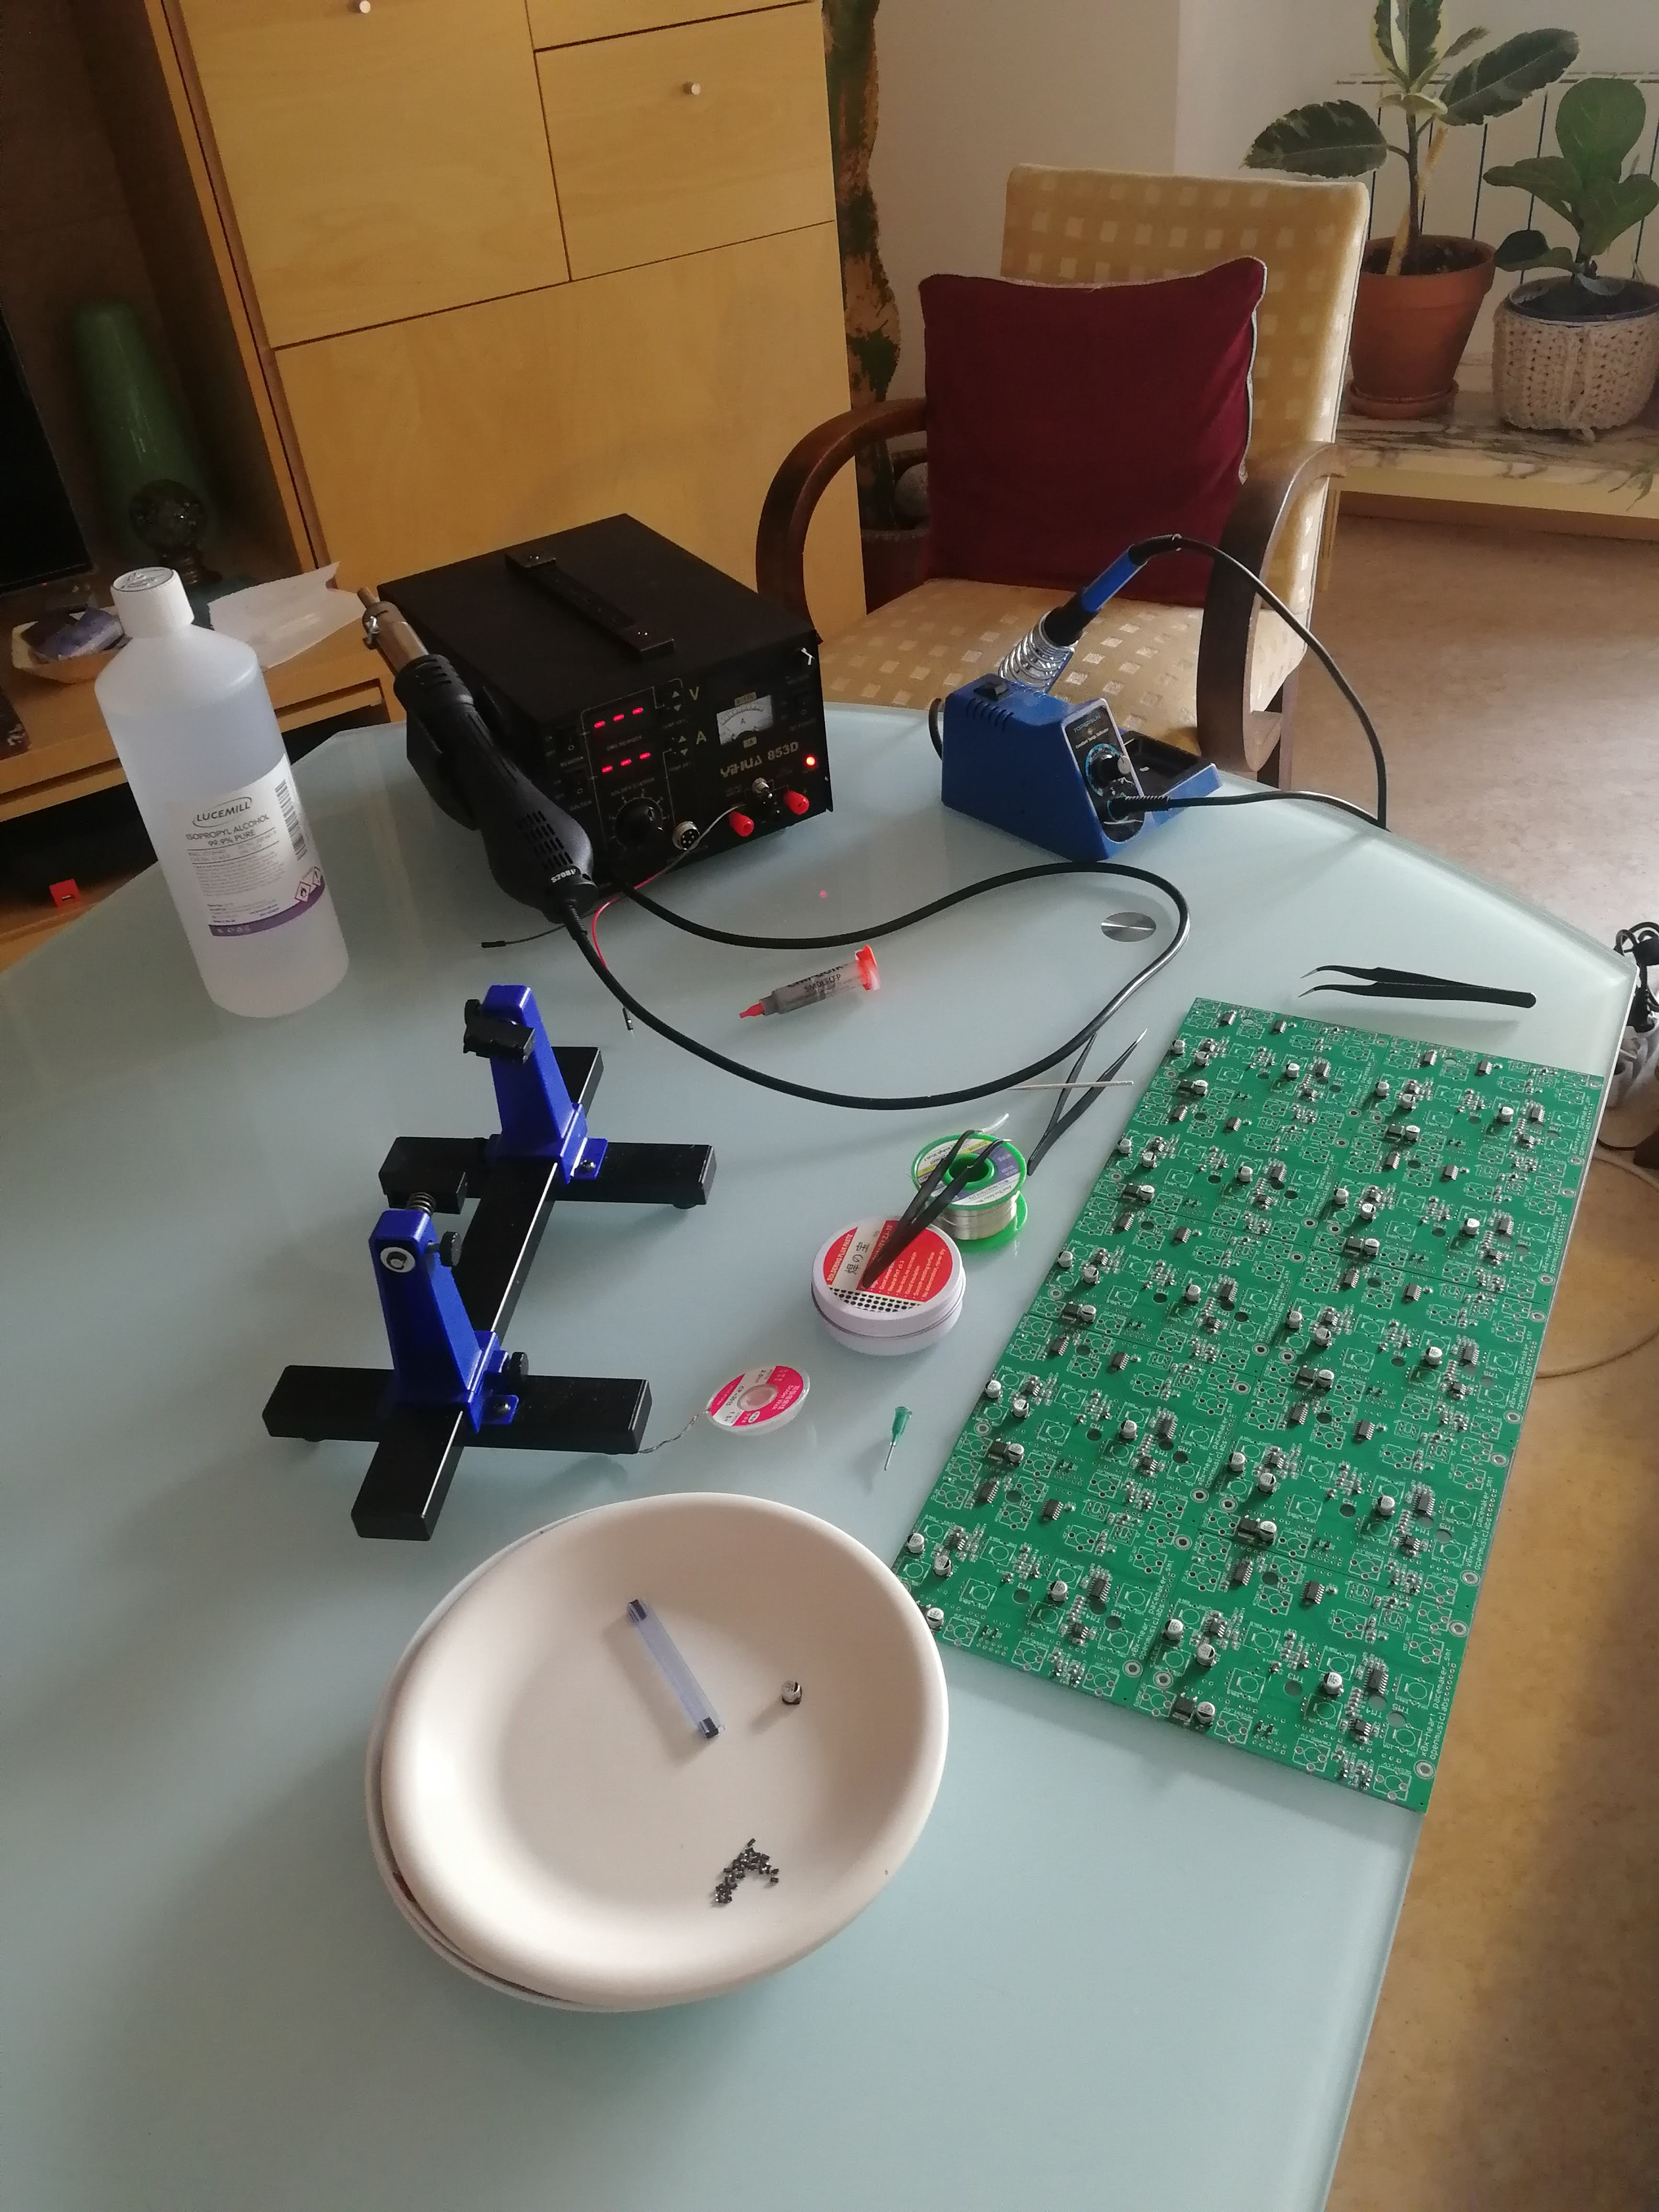
\includegraphics[width=0.92\textwidth]{atelier_maison1.jpg}
		%\caption{Proud of my weldings}
	\end{figure}
\end{column}
\begin{column}{0.65\textwidth}
	\begin{figure}[H]
		\centering
		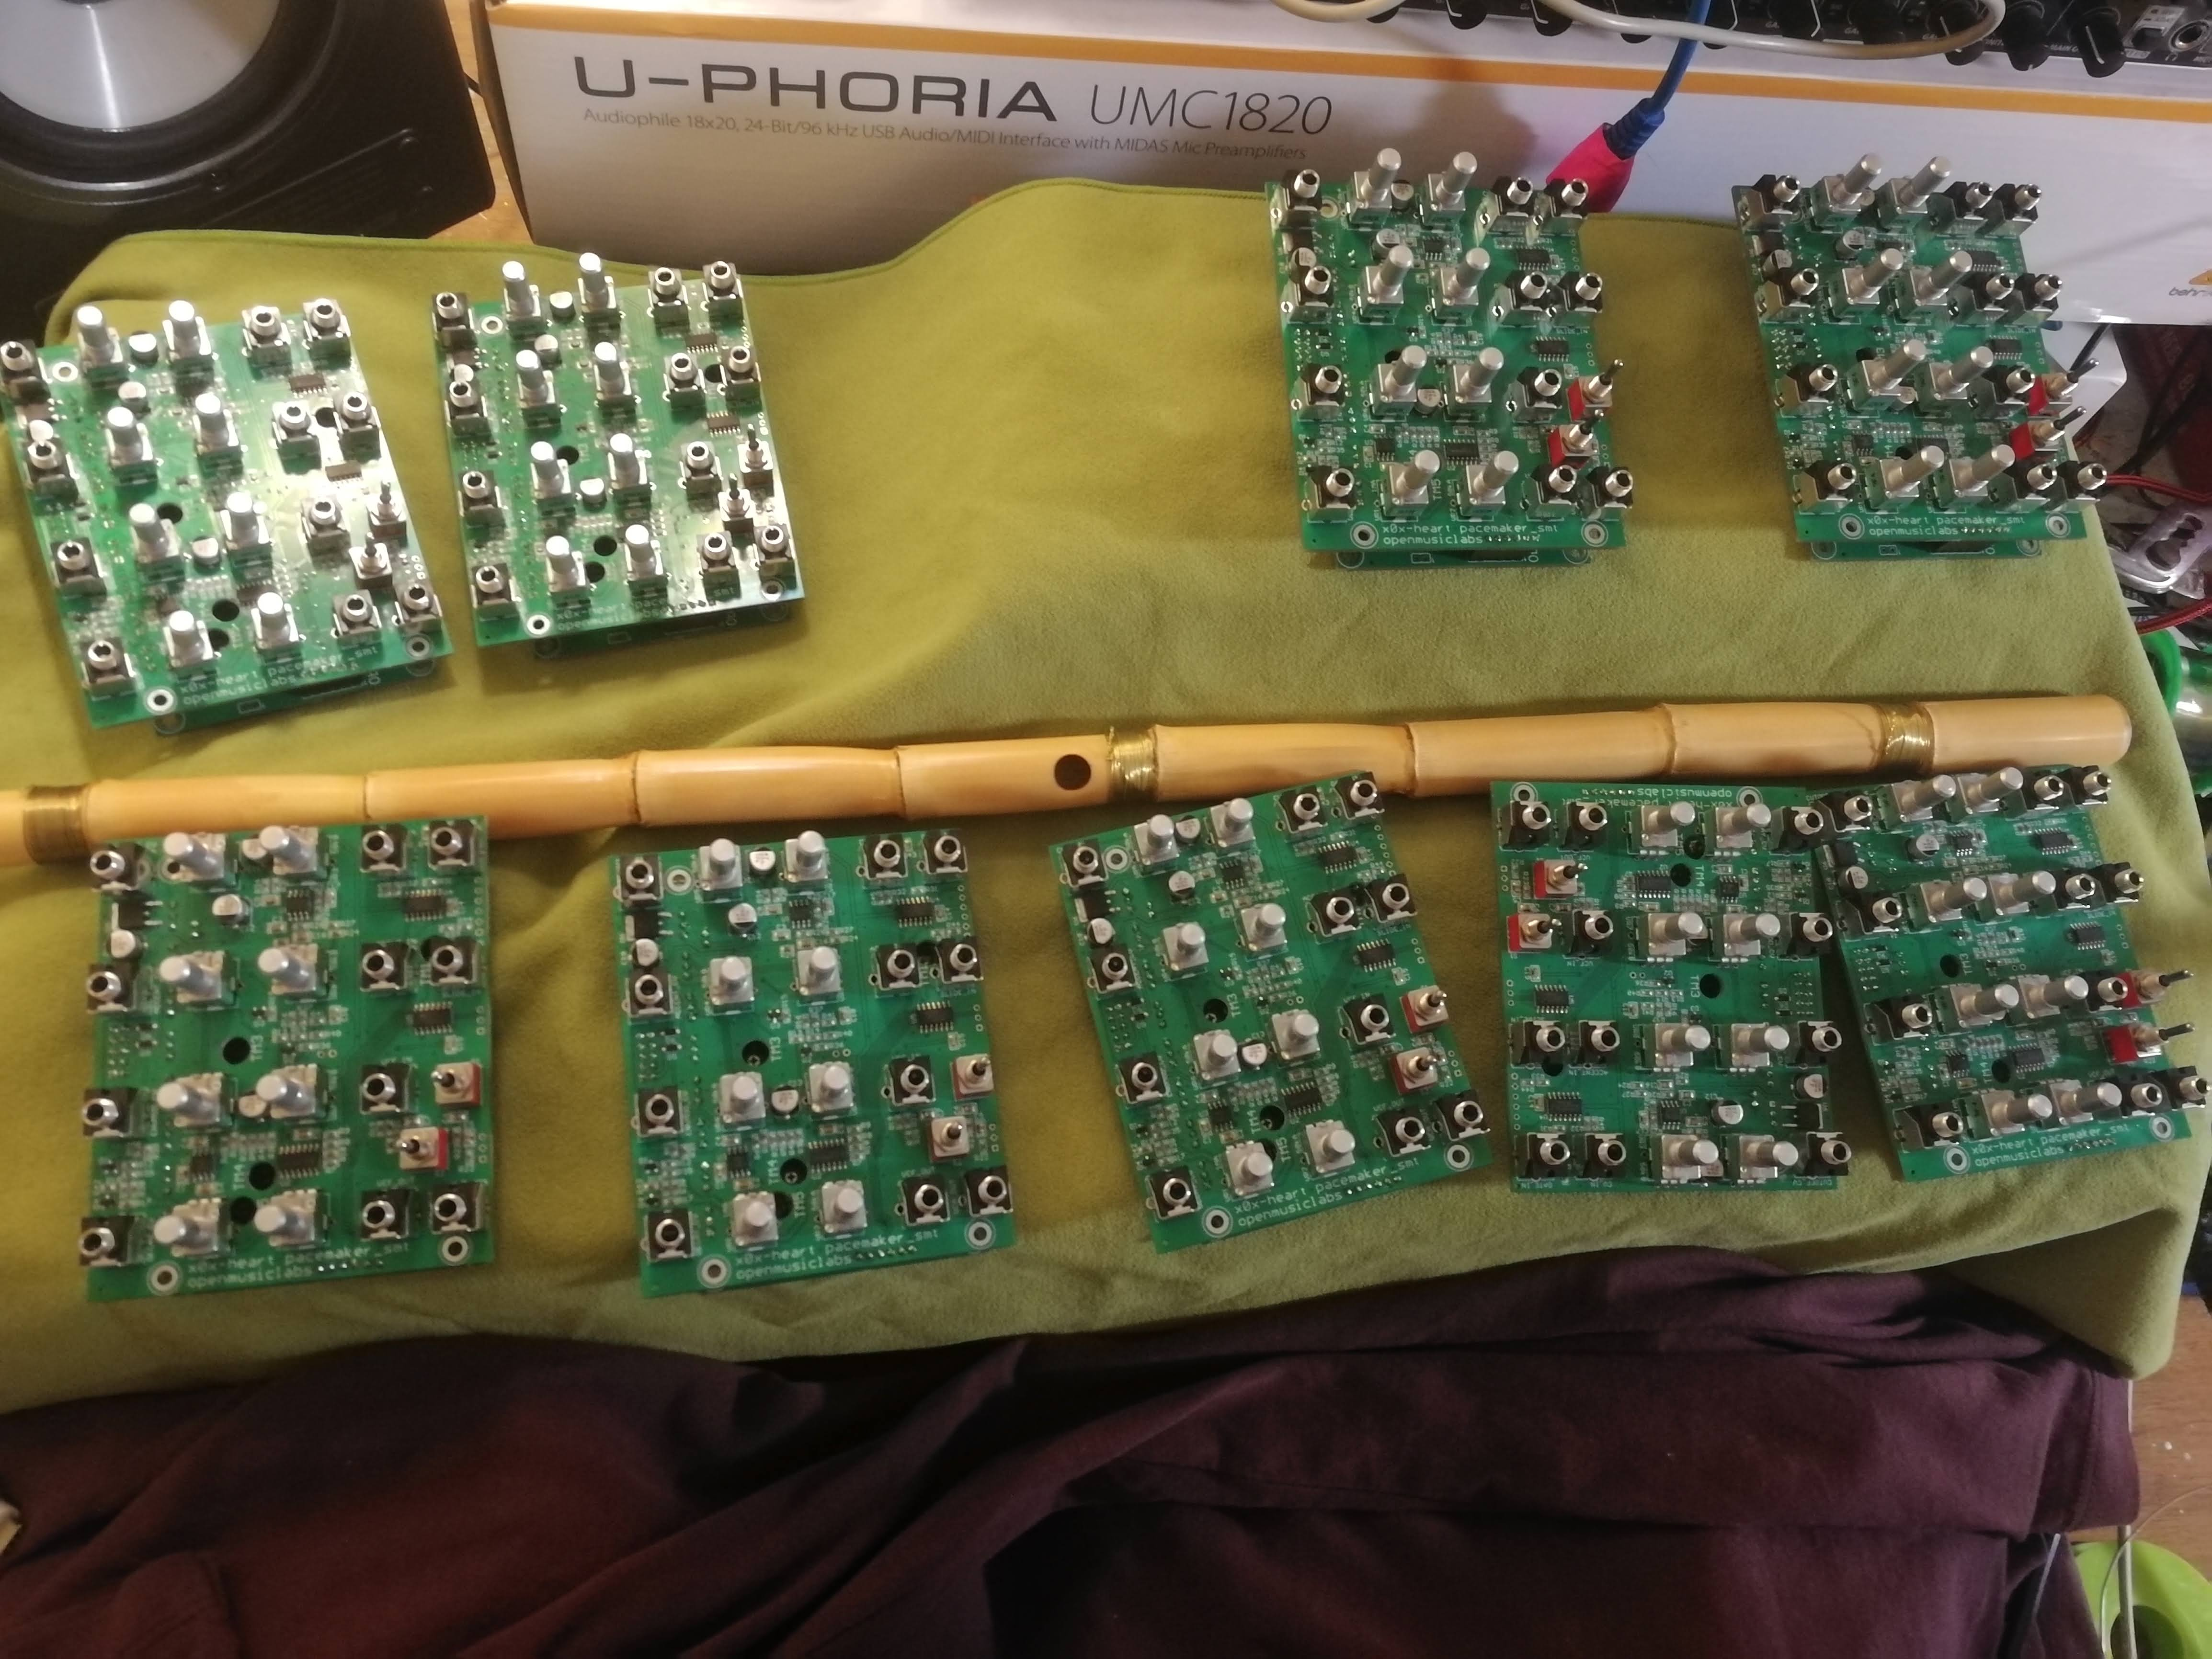
\includegraphics[width=0.9\textwidth]{atelier_maison2.jpg}
		%\caption{Proud of my weldings}
	\end{figure}
\end{column}
\end{columns}
\end{frame}

\begin{frame}
\frametitle{Custom Eurorack power modules}
\begin{columns}
\begin{column}{0.5\textwidth}
	\begin{figure}[H]
		\centering
		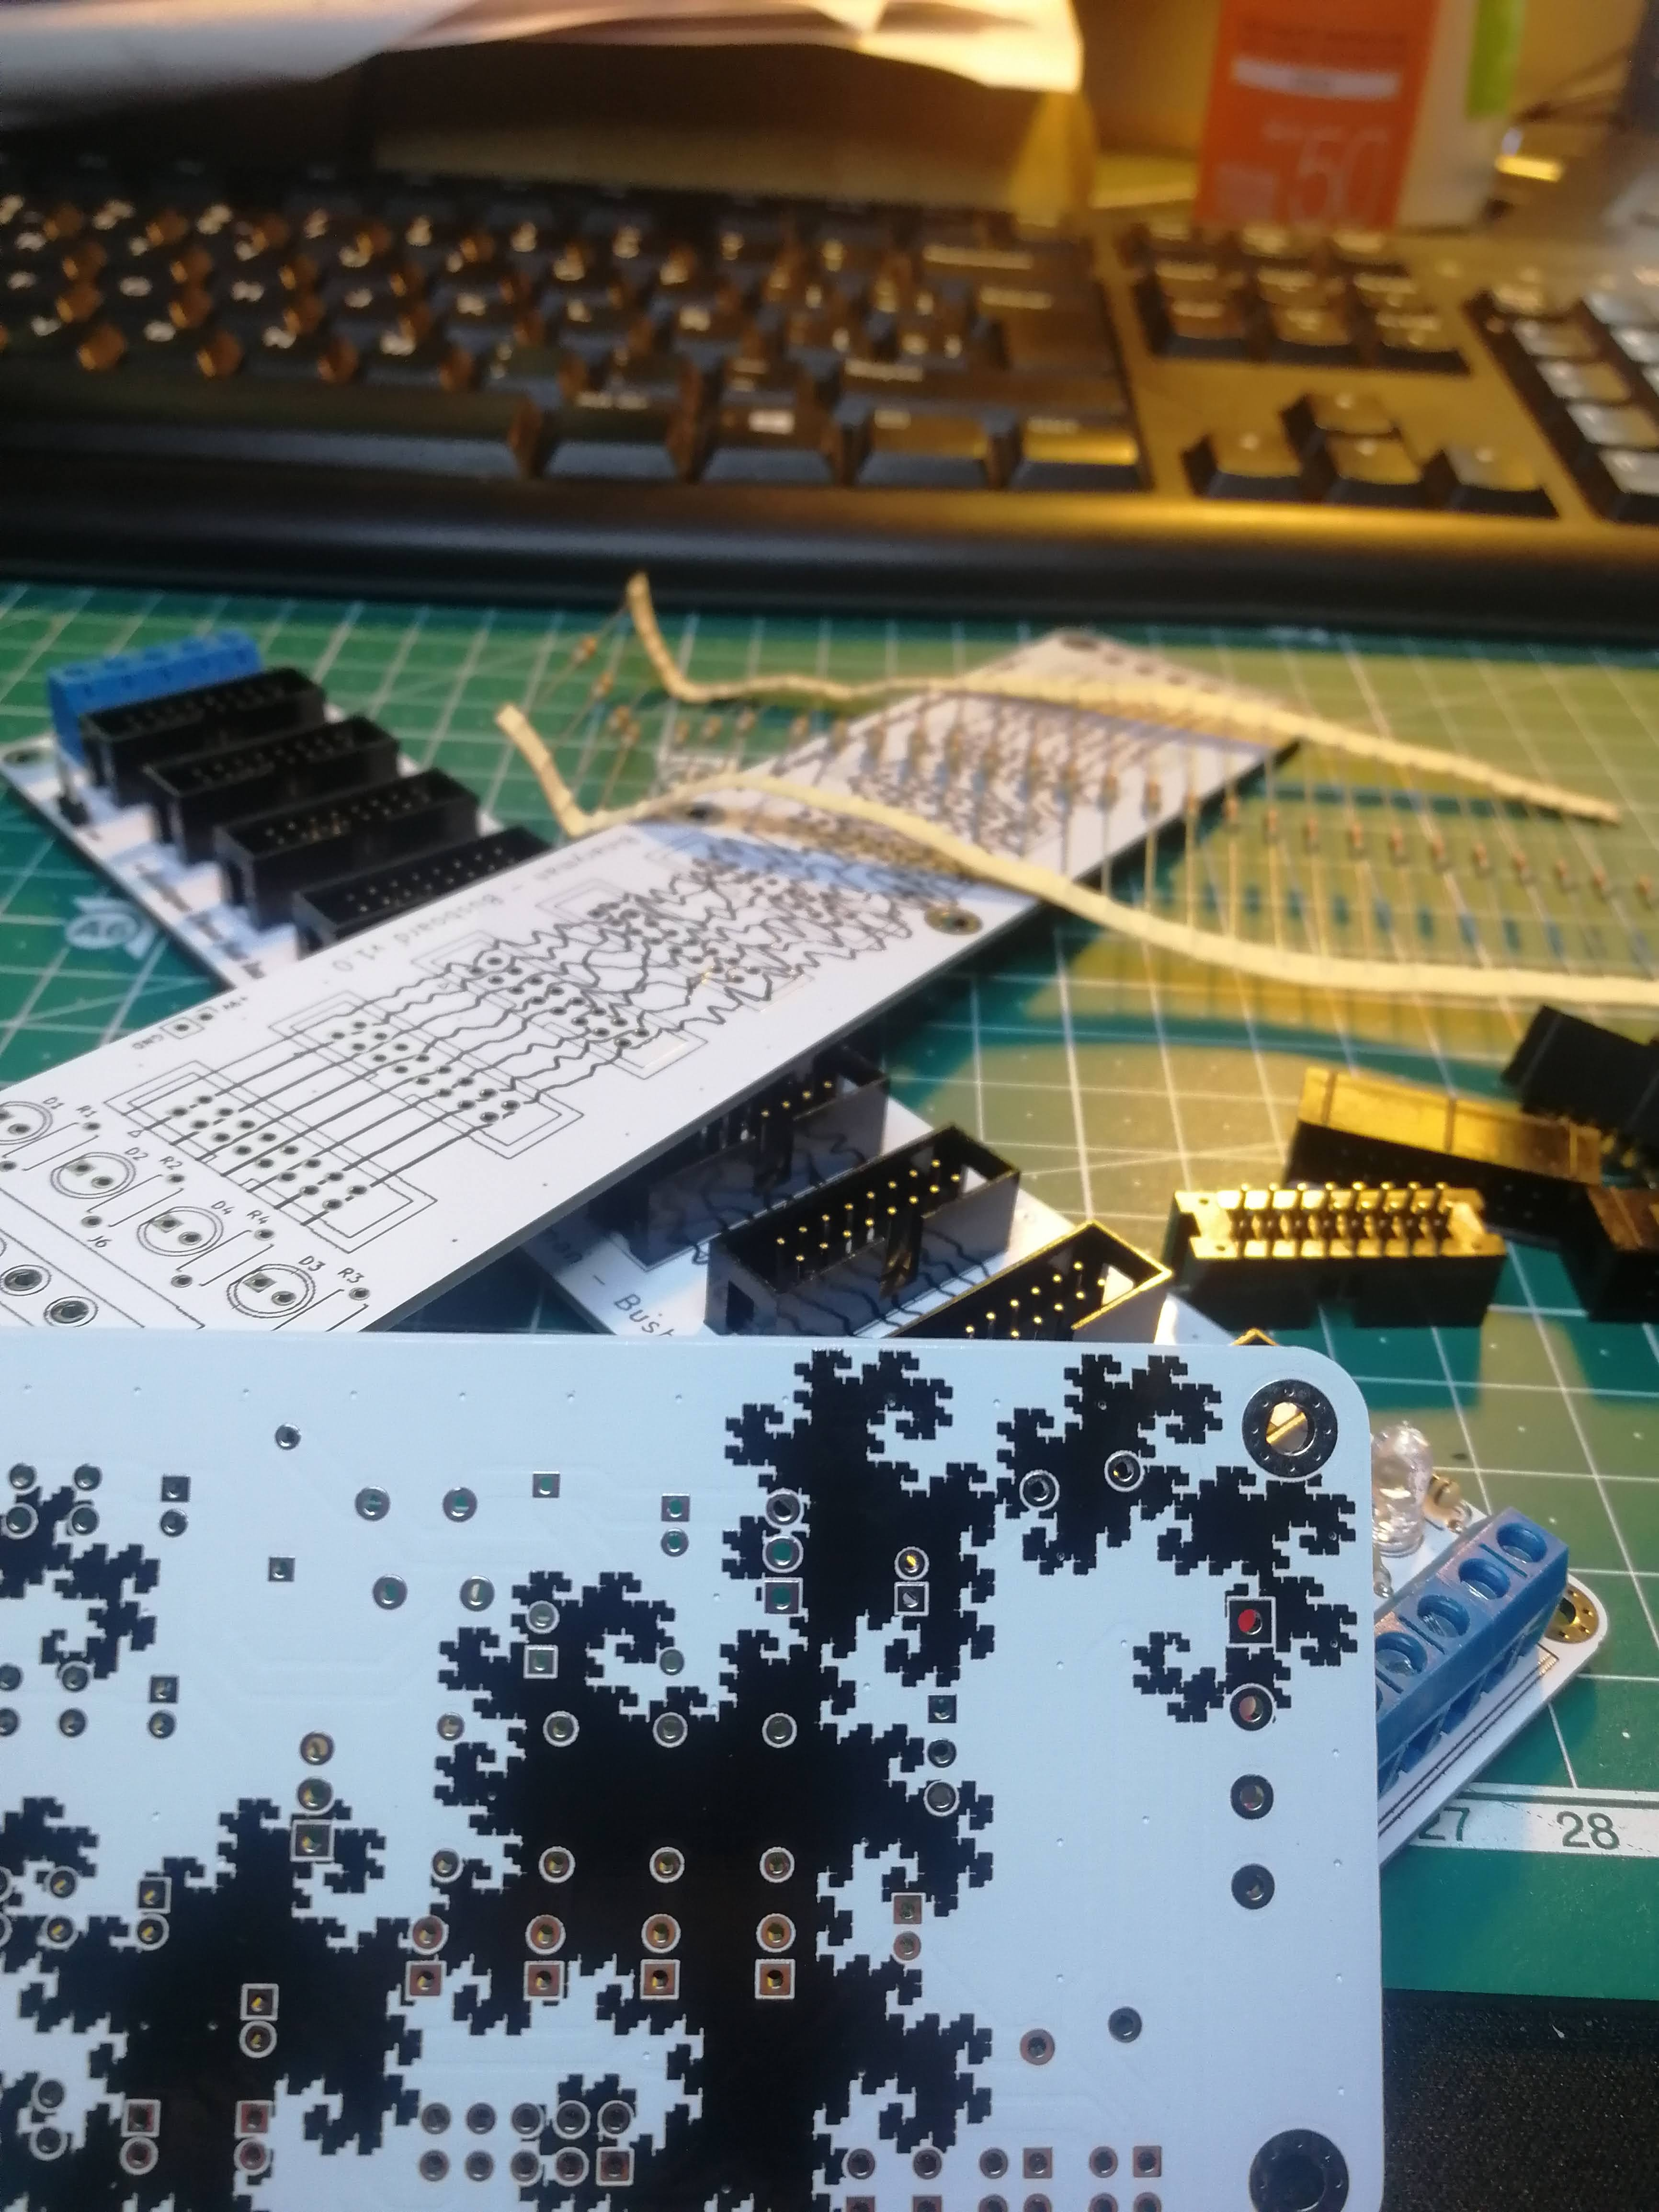
\includegraphics[width=0.8\textwidth]{eurorack1.jpg}
		%\caption{Proud of my weldings}
	\end{figure}
\end{column}
\begin{column}{0.5\textwidth}
	\begin{figure}[H]
		\centering
		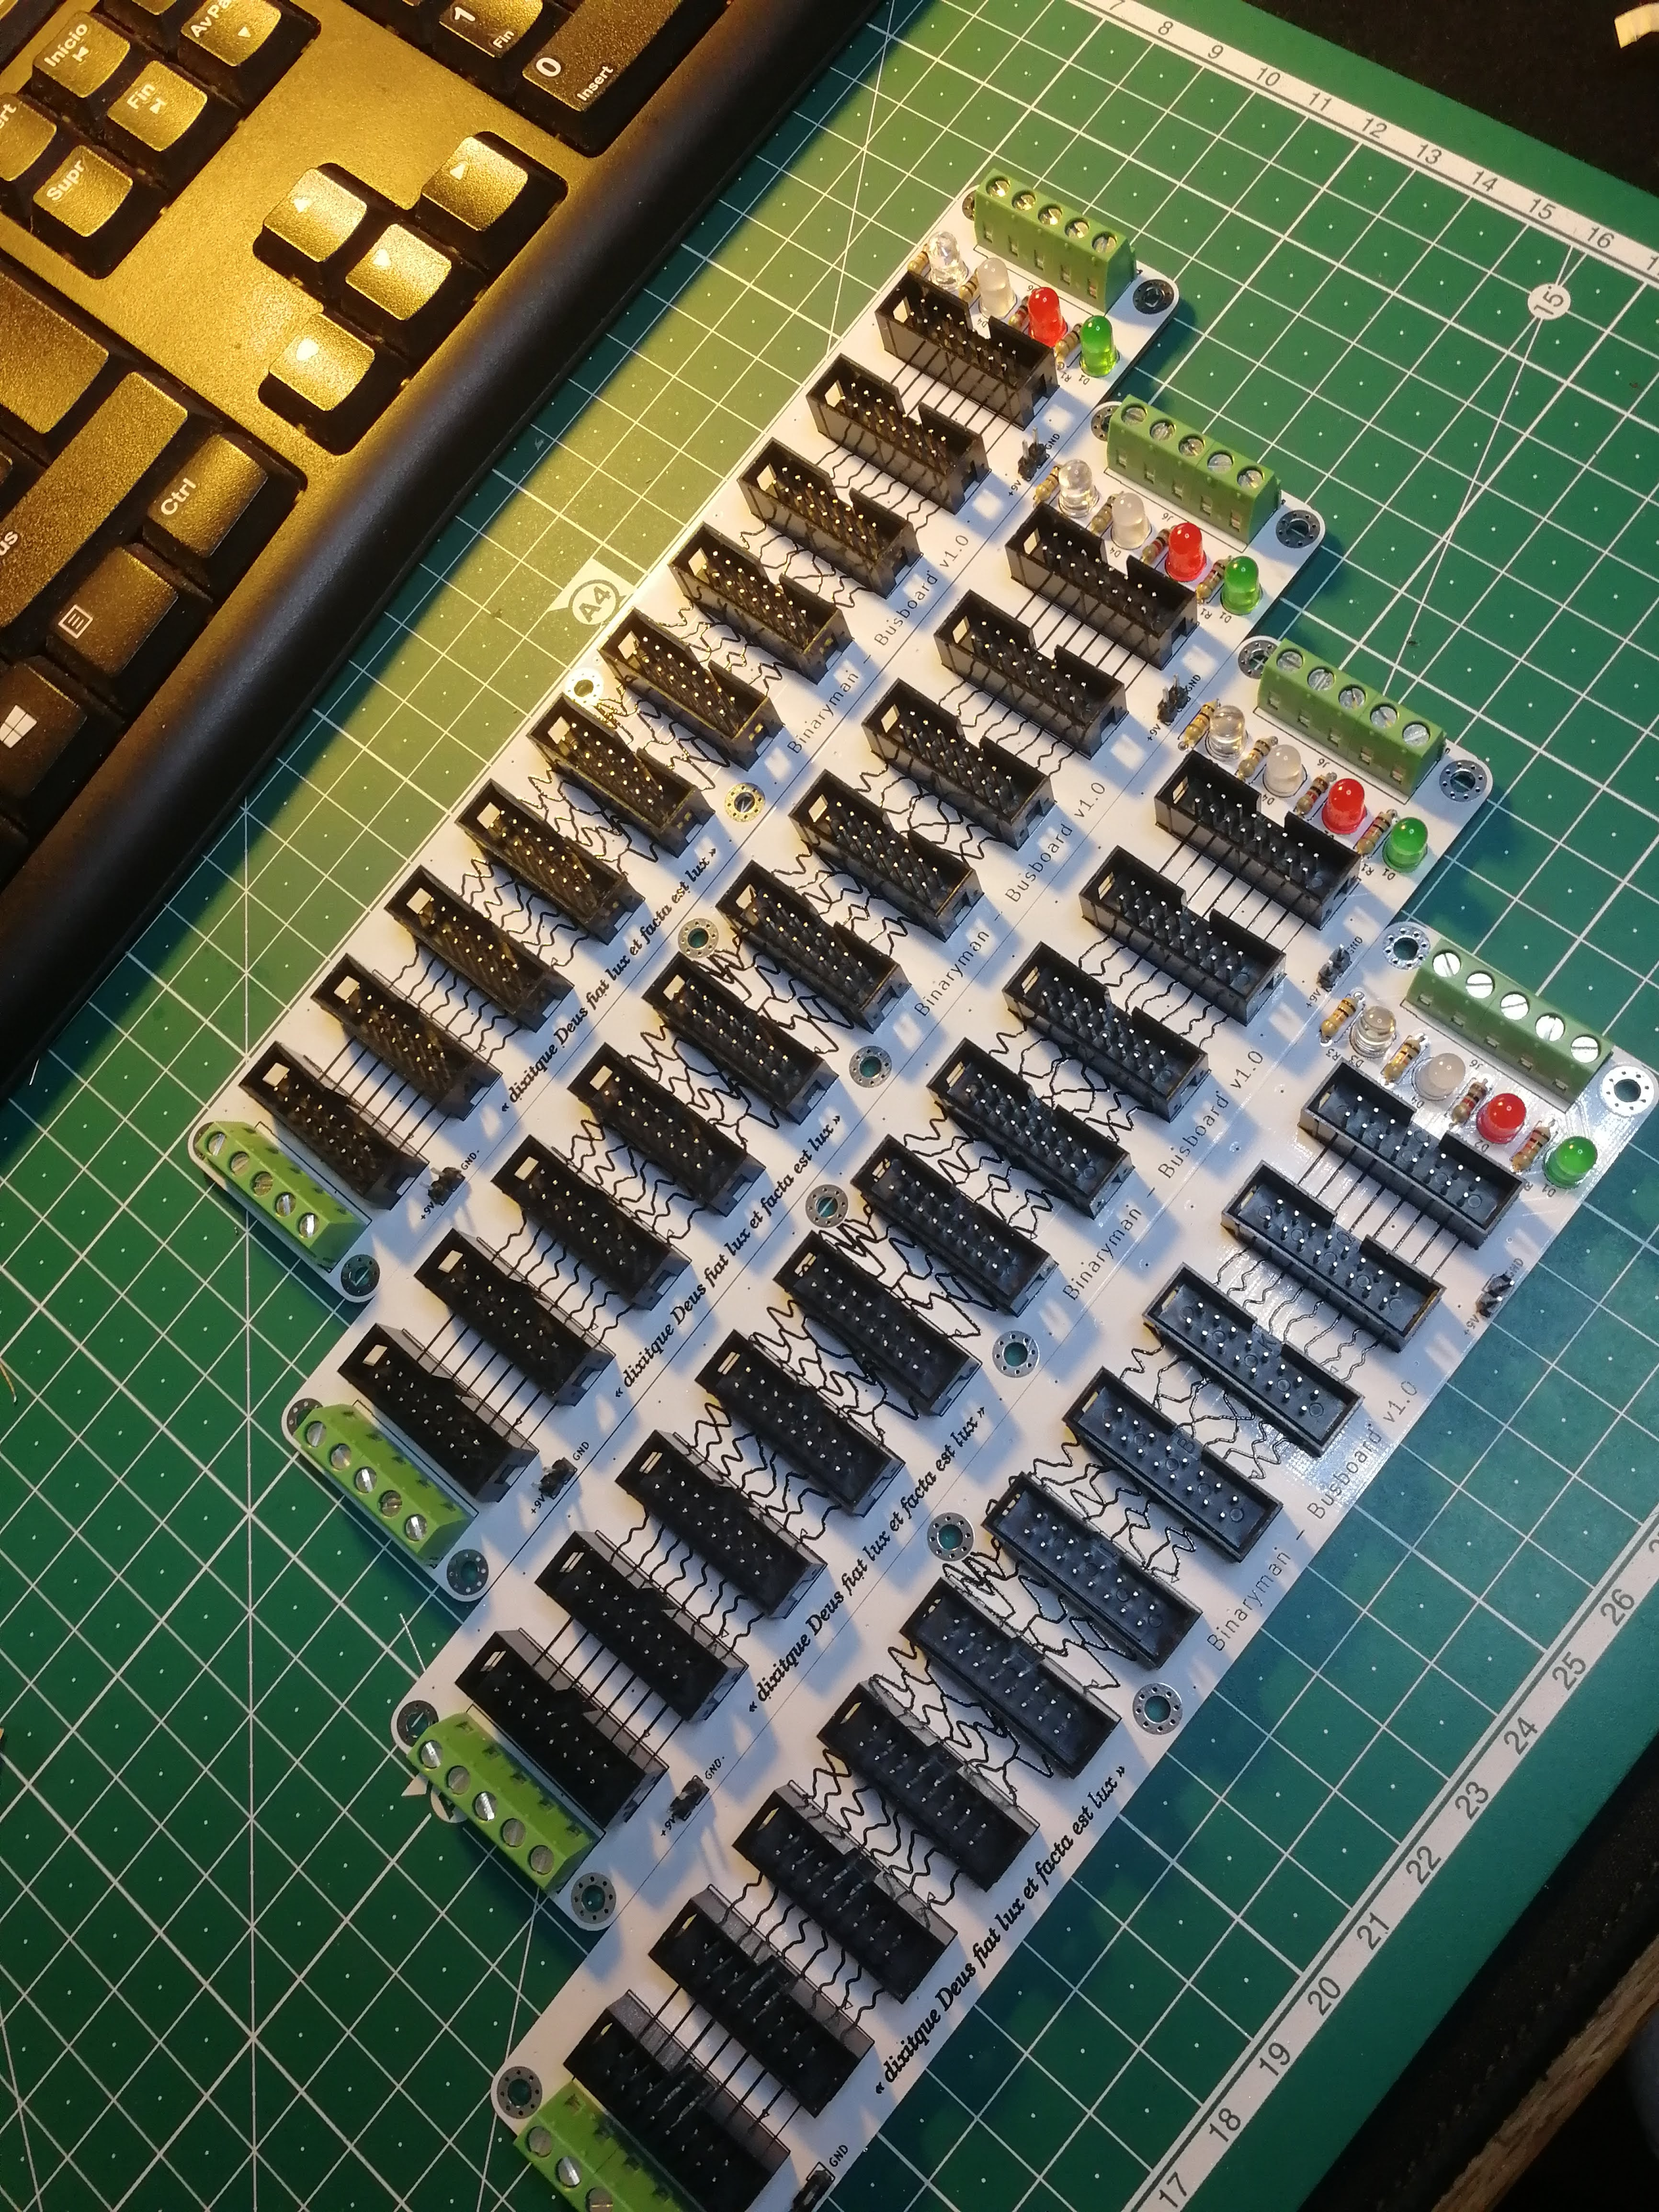
\includegraphics[width=0.8\textwidth]{eurorack2.jpg}
		%\caption{Proud of my weldings}
	\end{figure}
\end{column}
\end{columns}
\end{frame}

\begin{frame}
\frametitle{Custom Eurorack case}
\begin{columns}
\begin{column}{0.65\textwidth}
	\begin{figure}[H]
		\centering
		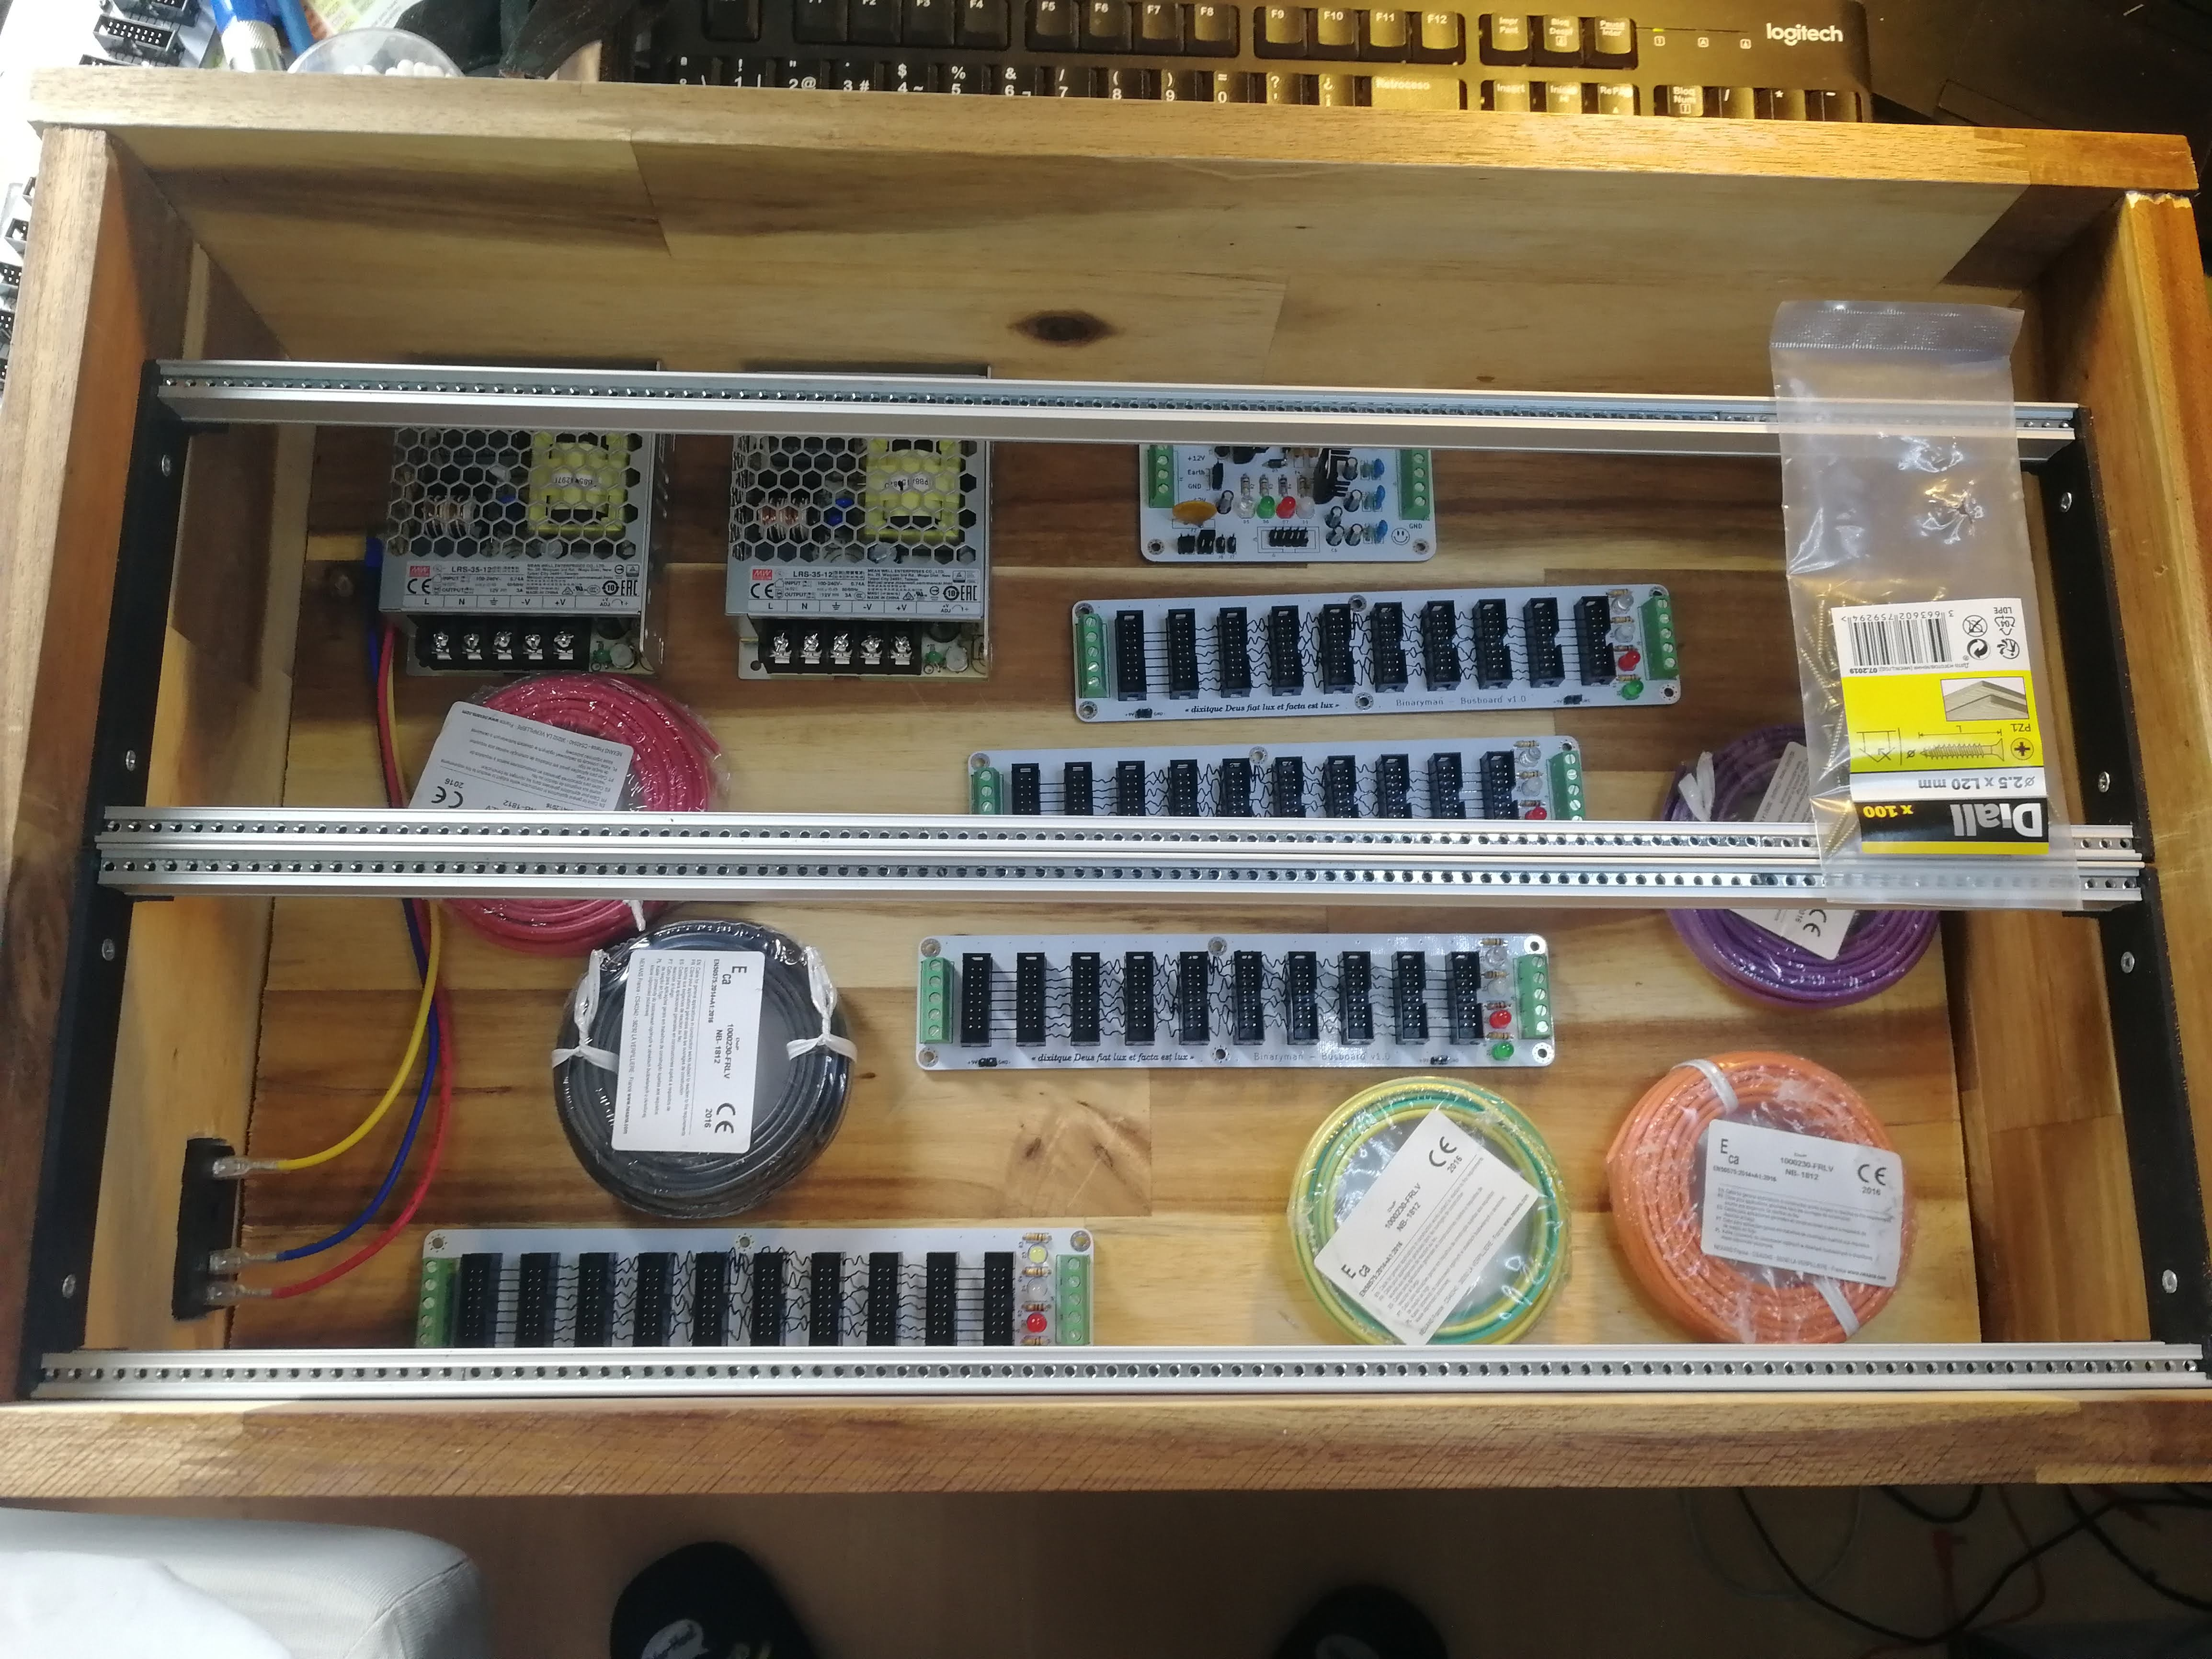
\includegraphics[width=0.86\textwidth]{eurorack3.jpg}
		%\caption{Proud of my weldings}
	\end{figure}
\end{column}
\begin{column}{0.35\textwidth}
	\begin{figure}[H]
		\centering
		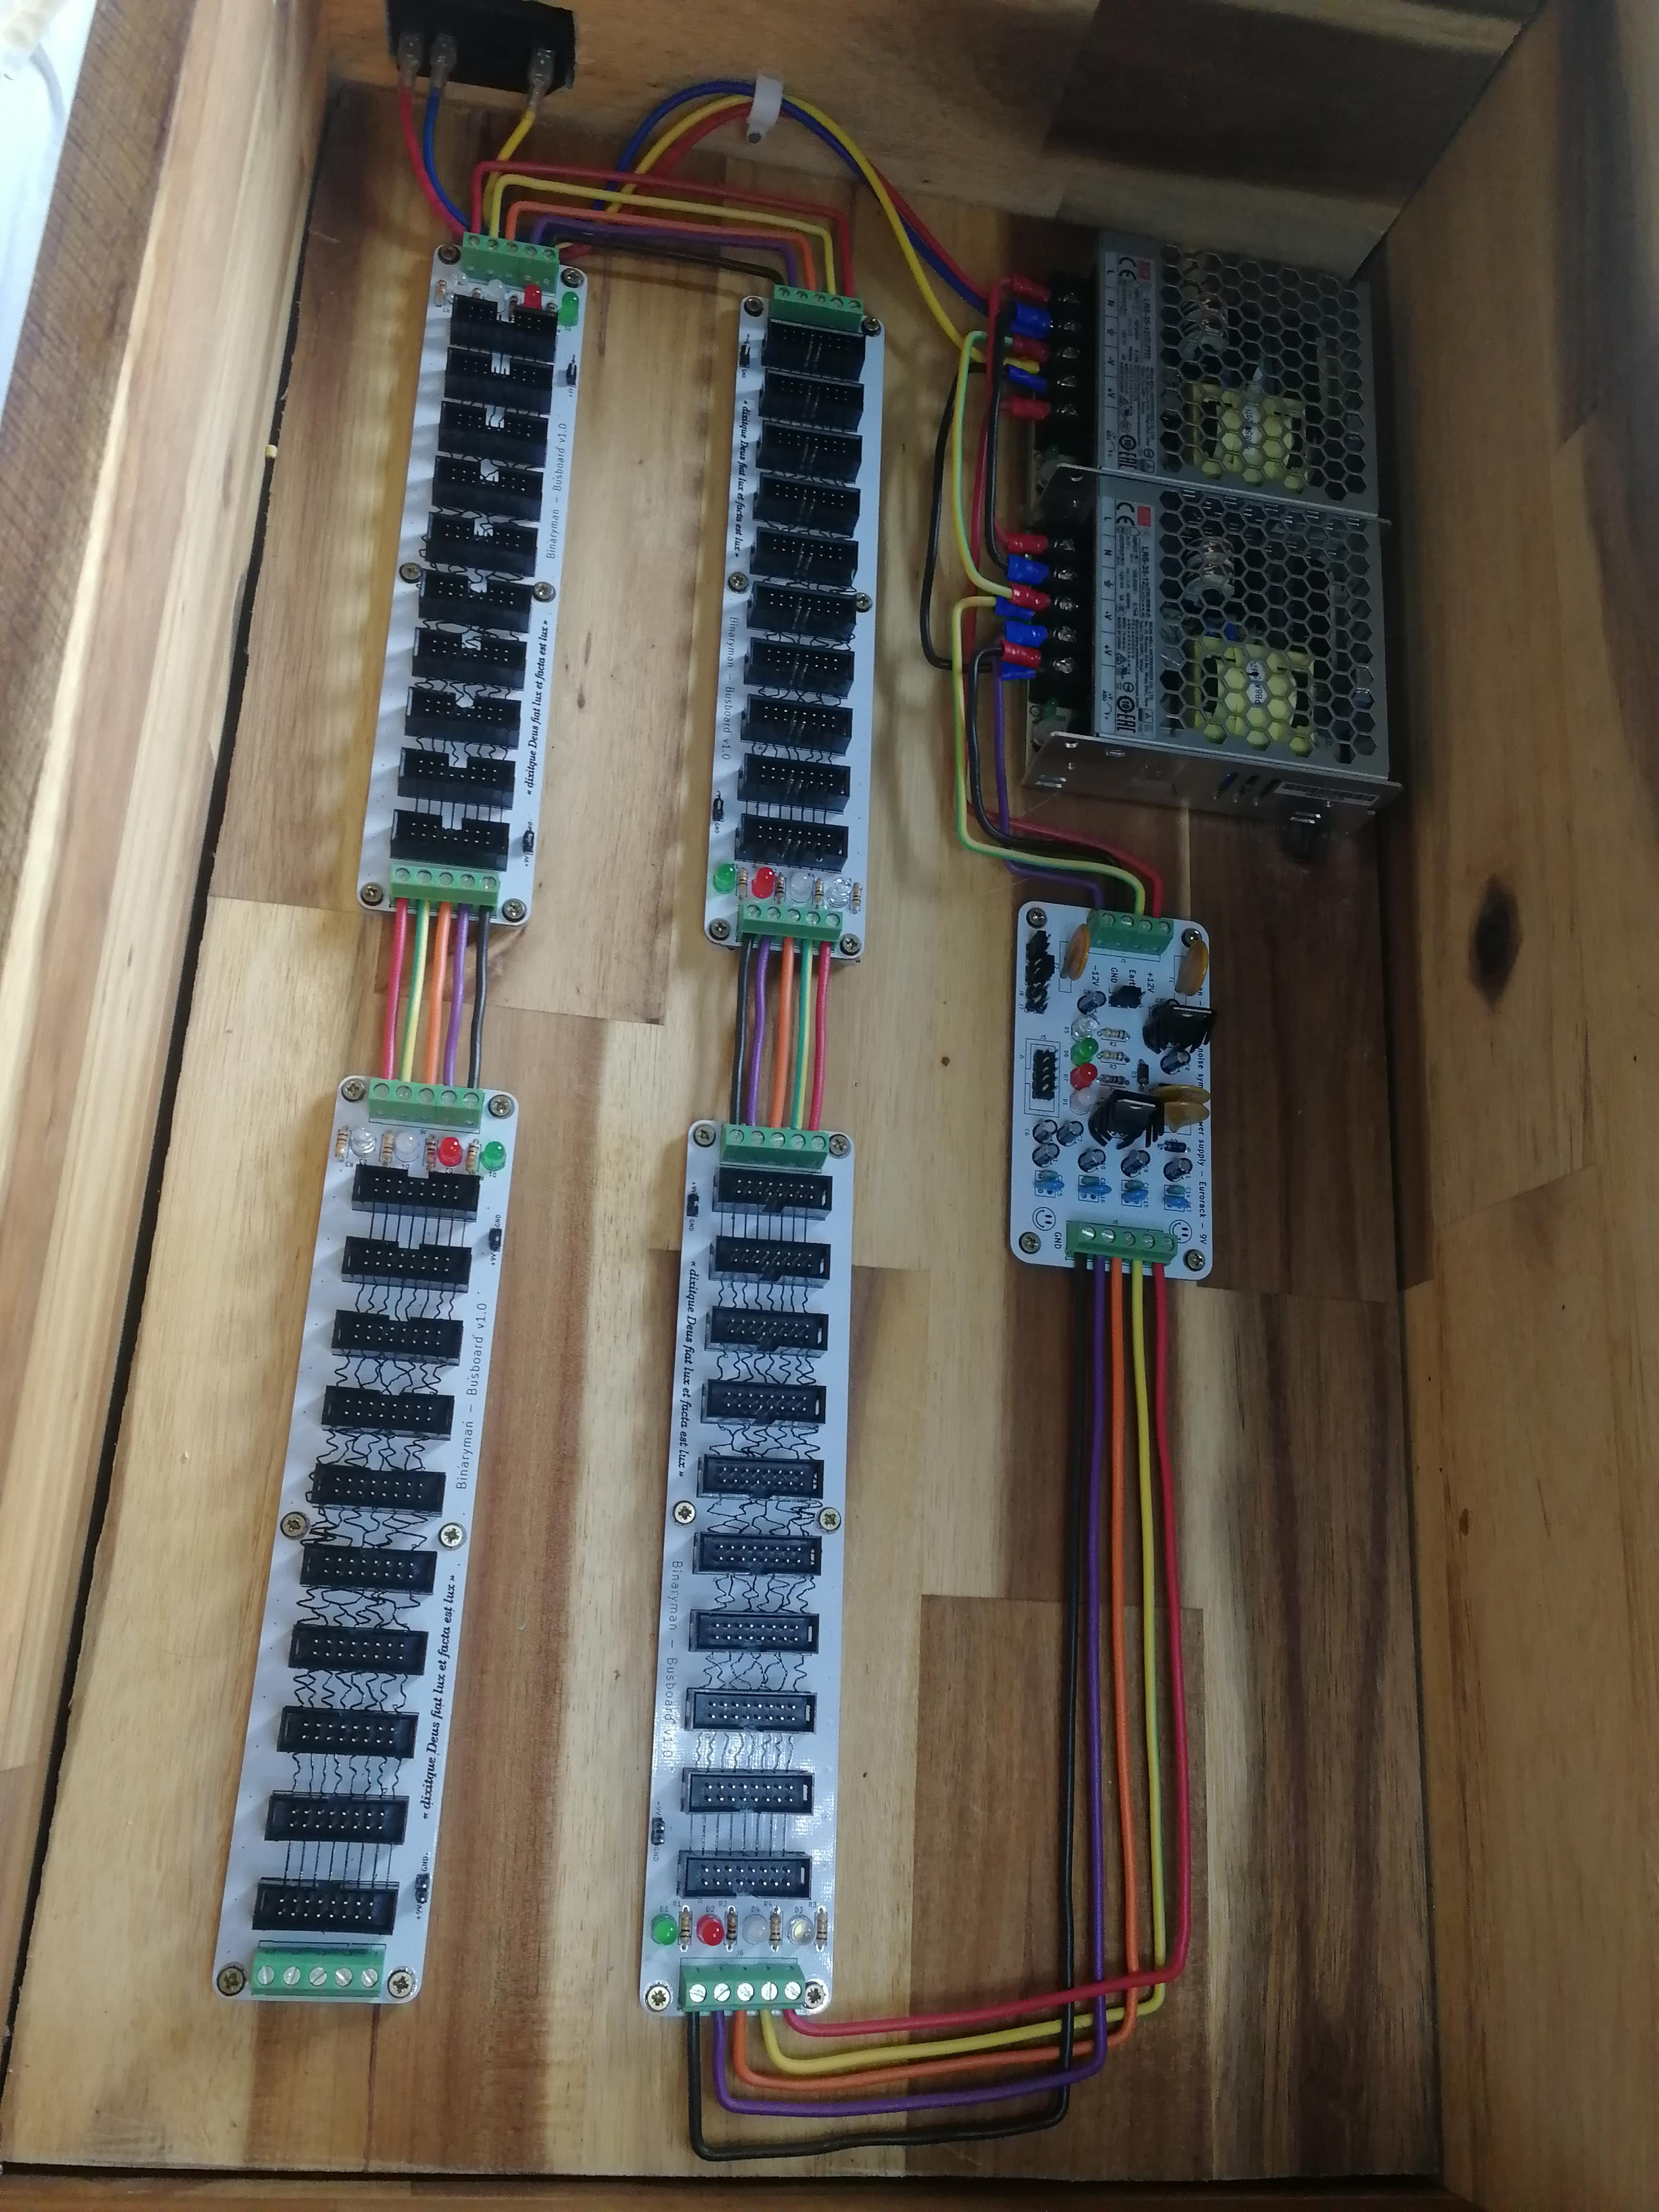
\includegraphics[width=0.9\textwidth]{eurorack4.jpg}
		%\caption{Proud of my weldings}
	\end{figure}
\end{column}
\end{columns}
\end{frame}

\begin{frame}
\frametitle{Flopotron / RetrOrchestre}
\begin{columns}
\begin{column}{0.35\textwidth}
	\begin{figure}[H]
		\centering
		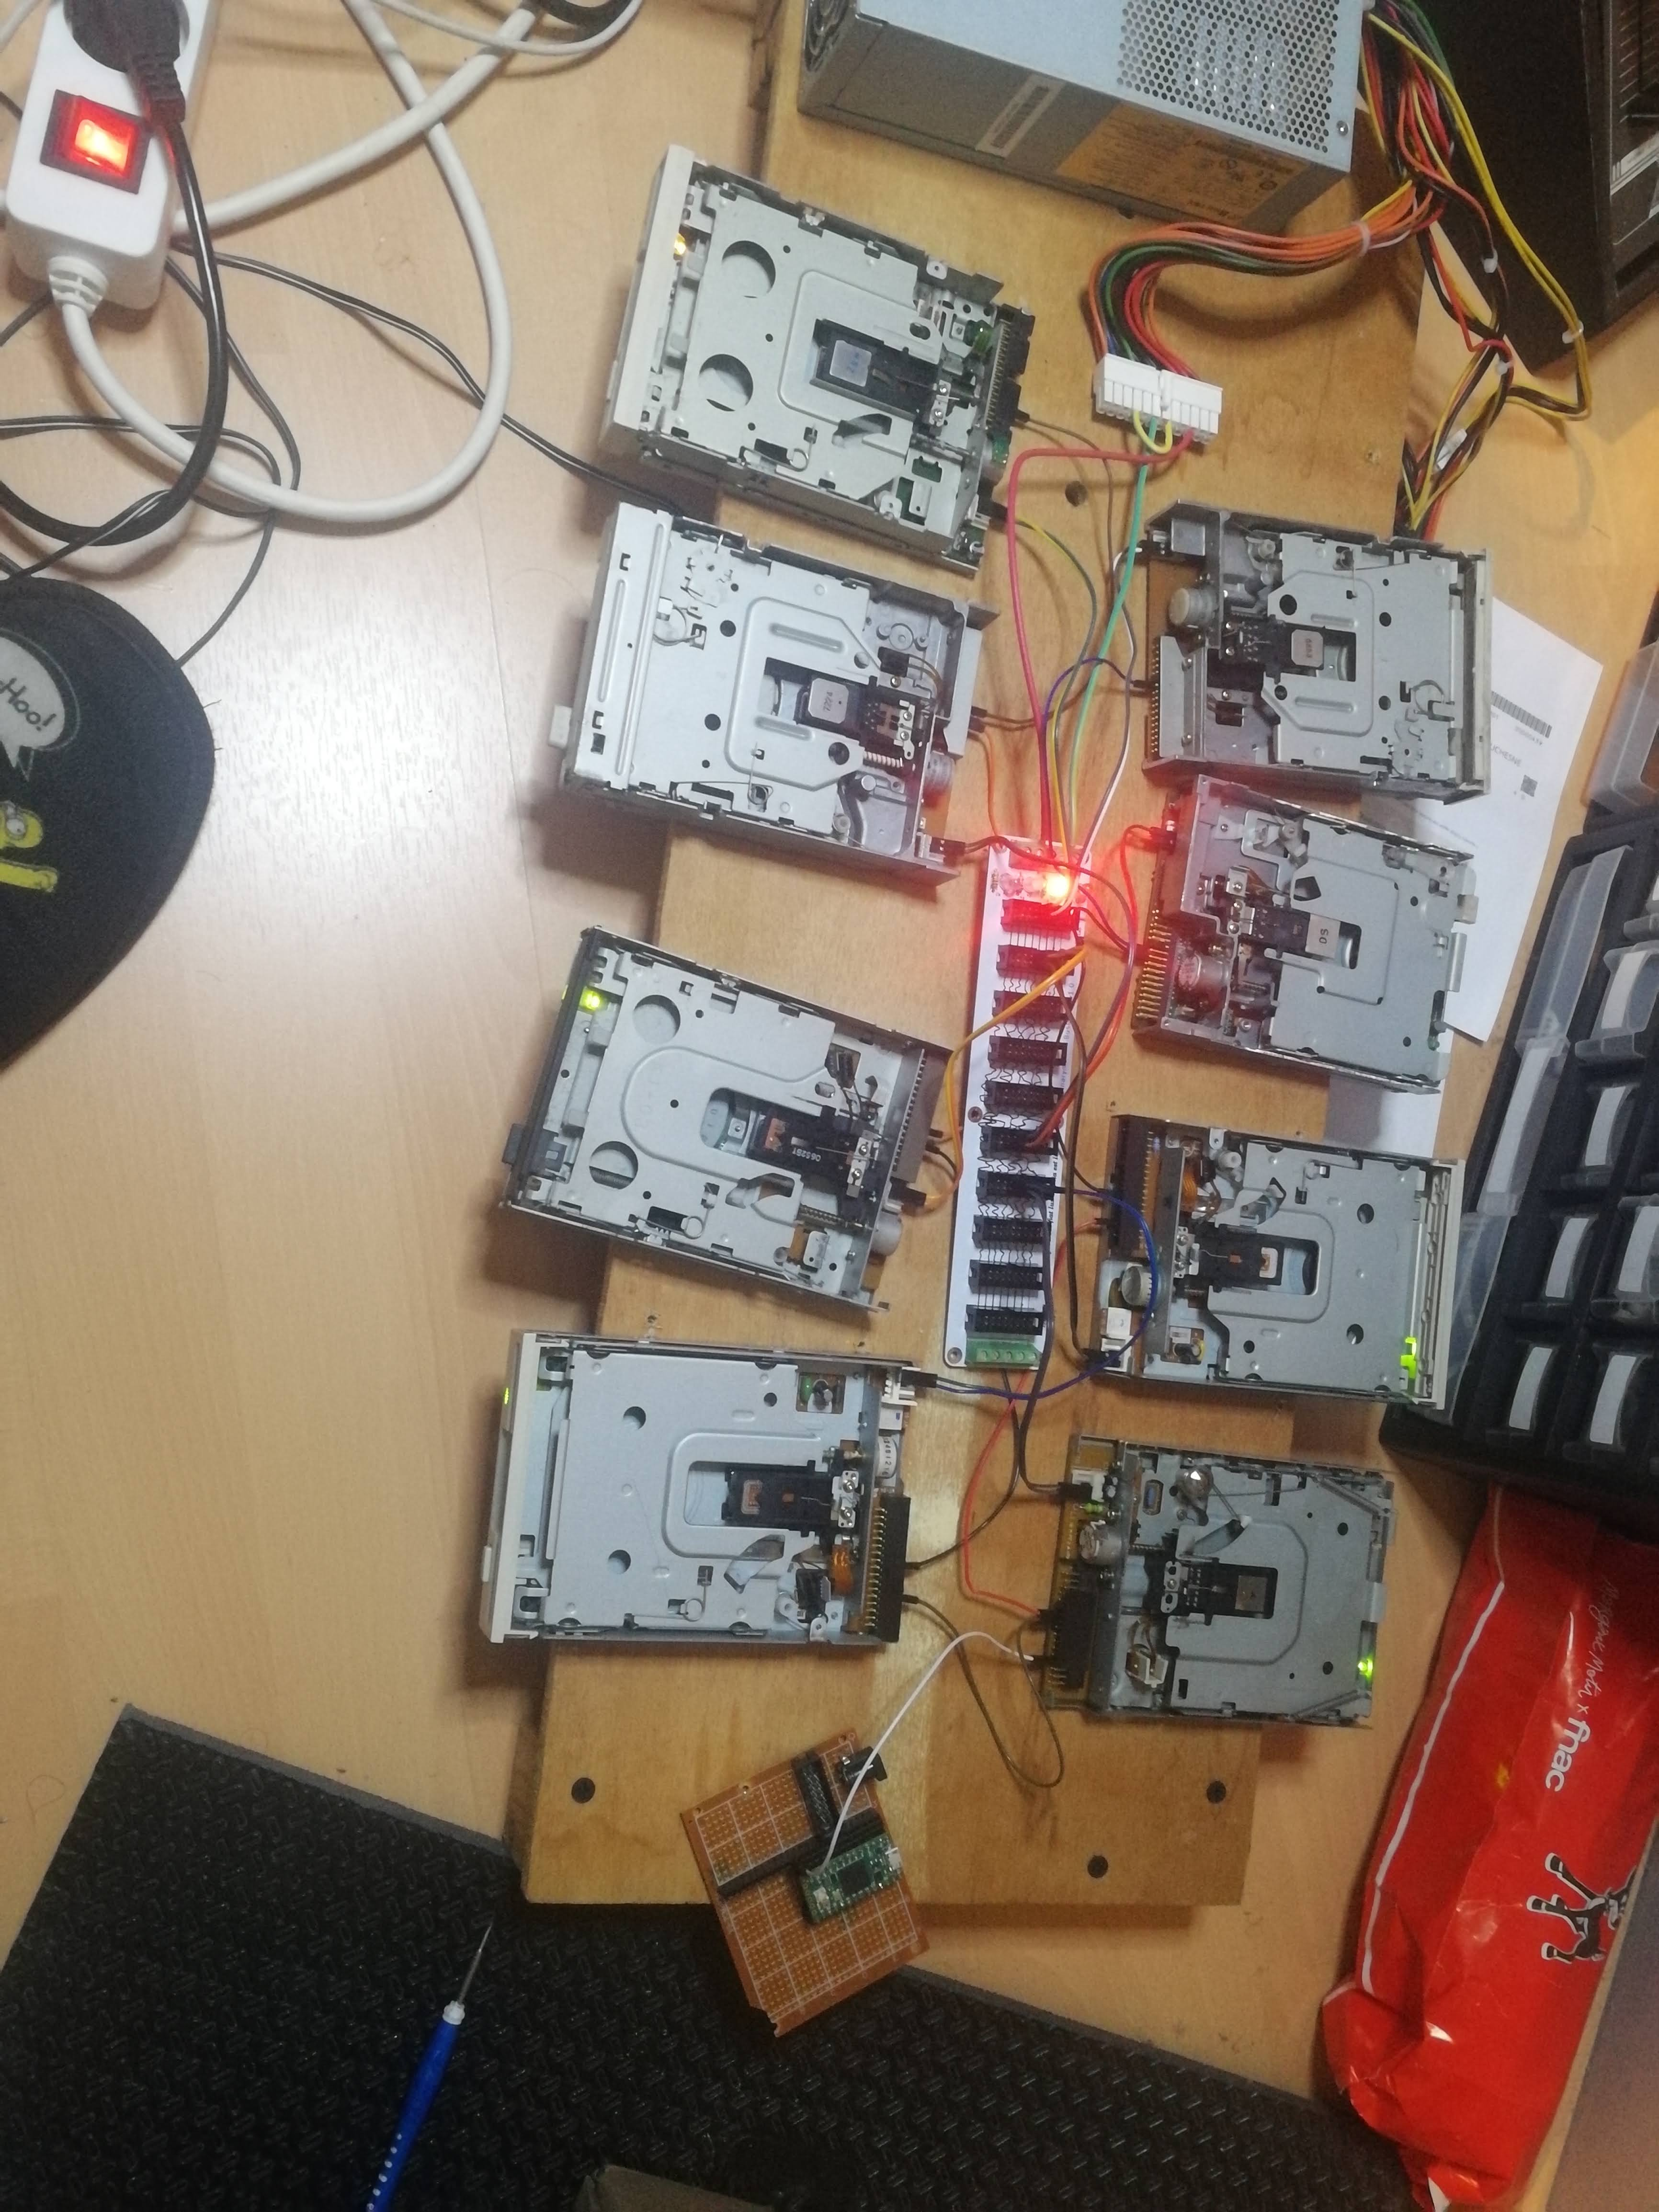
\includegraphics[width=0.9\textwidth]{flopotron1.jpg}
		%\caption{Proud of my weldings}
	\end{figure}
\end{column}
\begin{column}{0.65\textwidth}
	\begin{figure}[H]
		\centering
		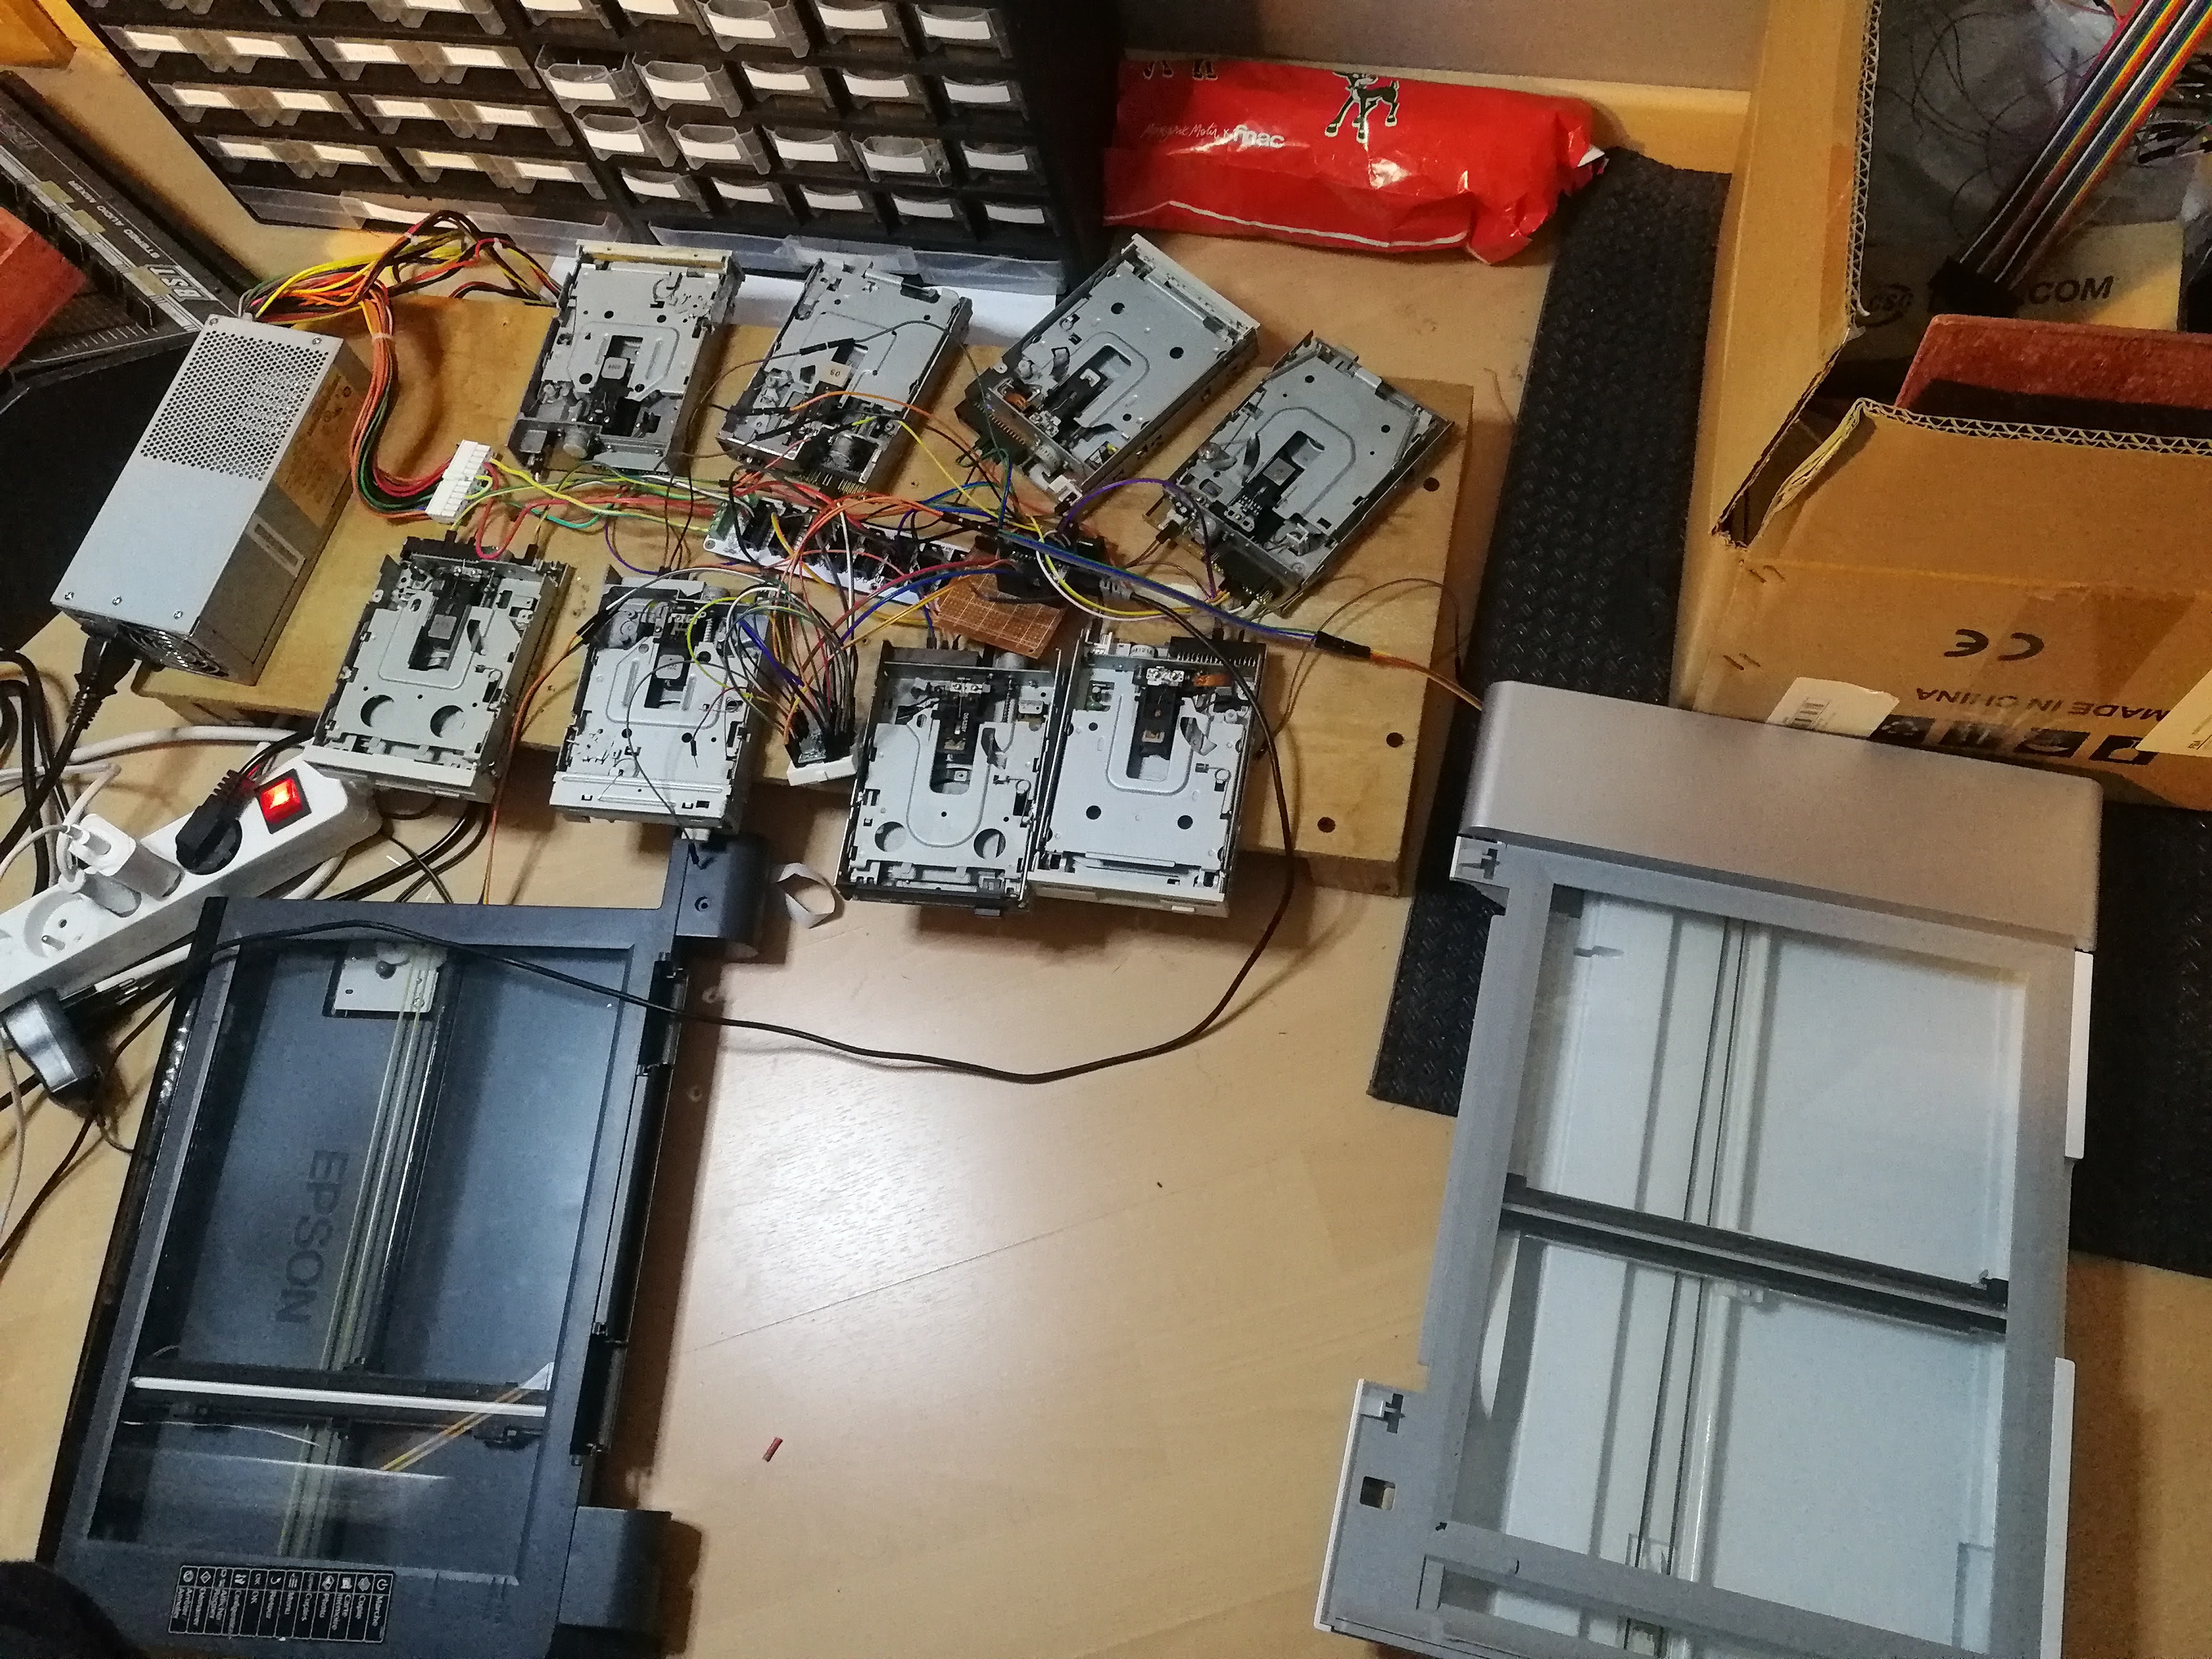
\includegraphics[width=0.86\textwidth]{flopotron2.jpg}
		%\caption{Proud of my weldings}
	\end{figure}
\end{column}
\end{columns}
\end{frame}

\begin{frame}
\frametitle{It started long time ago..}
\begin{columns}
\begin{column}{0.6\textwidth}
	\begin{figure}[H]
		\centering
		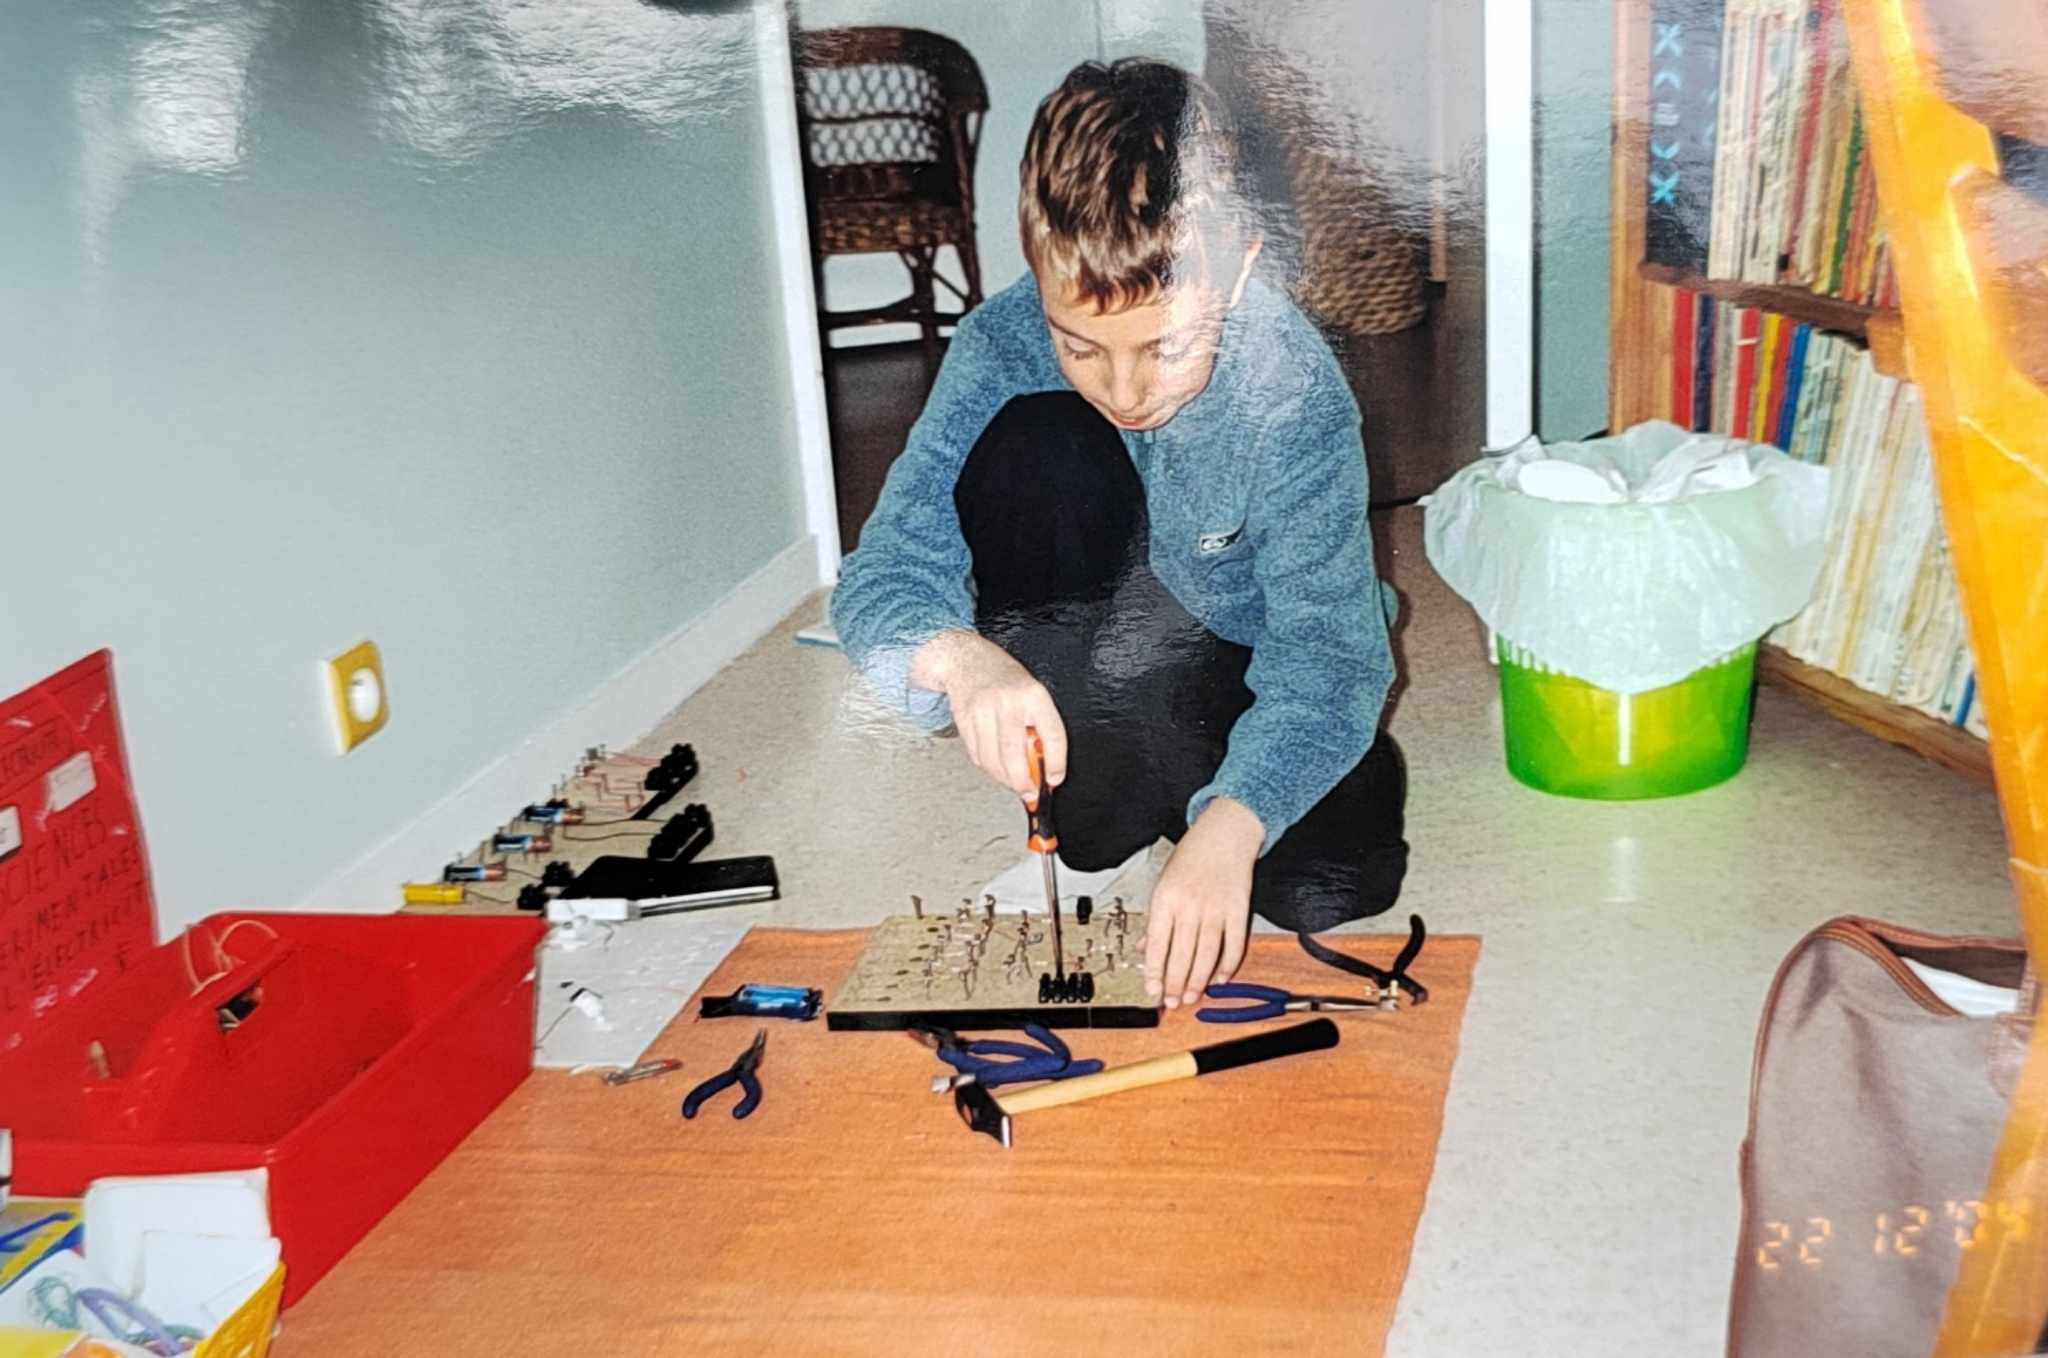
\includegraphics[width=\textwidth]{moi1.jpg}
		%\caption{Proud of my weldings}
	\end{figure}
\end{column}
\begin{column}{0.4\textwidth}
	\begin{figure}[H]
		\centering
		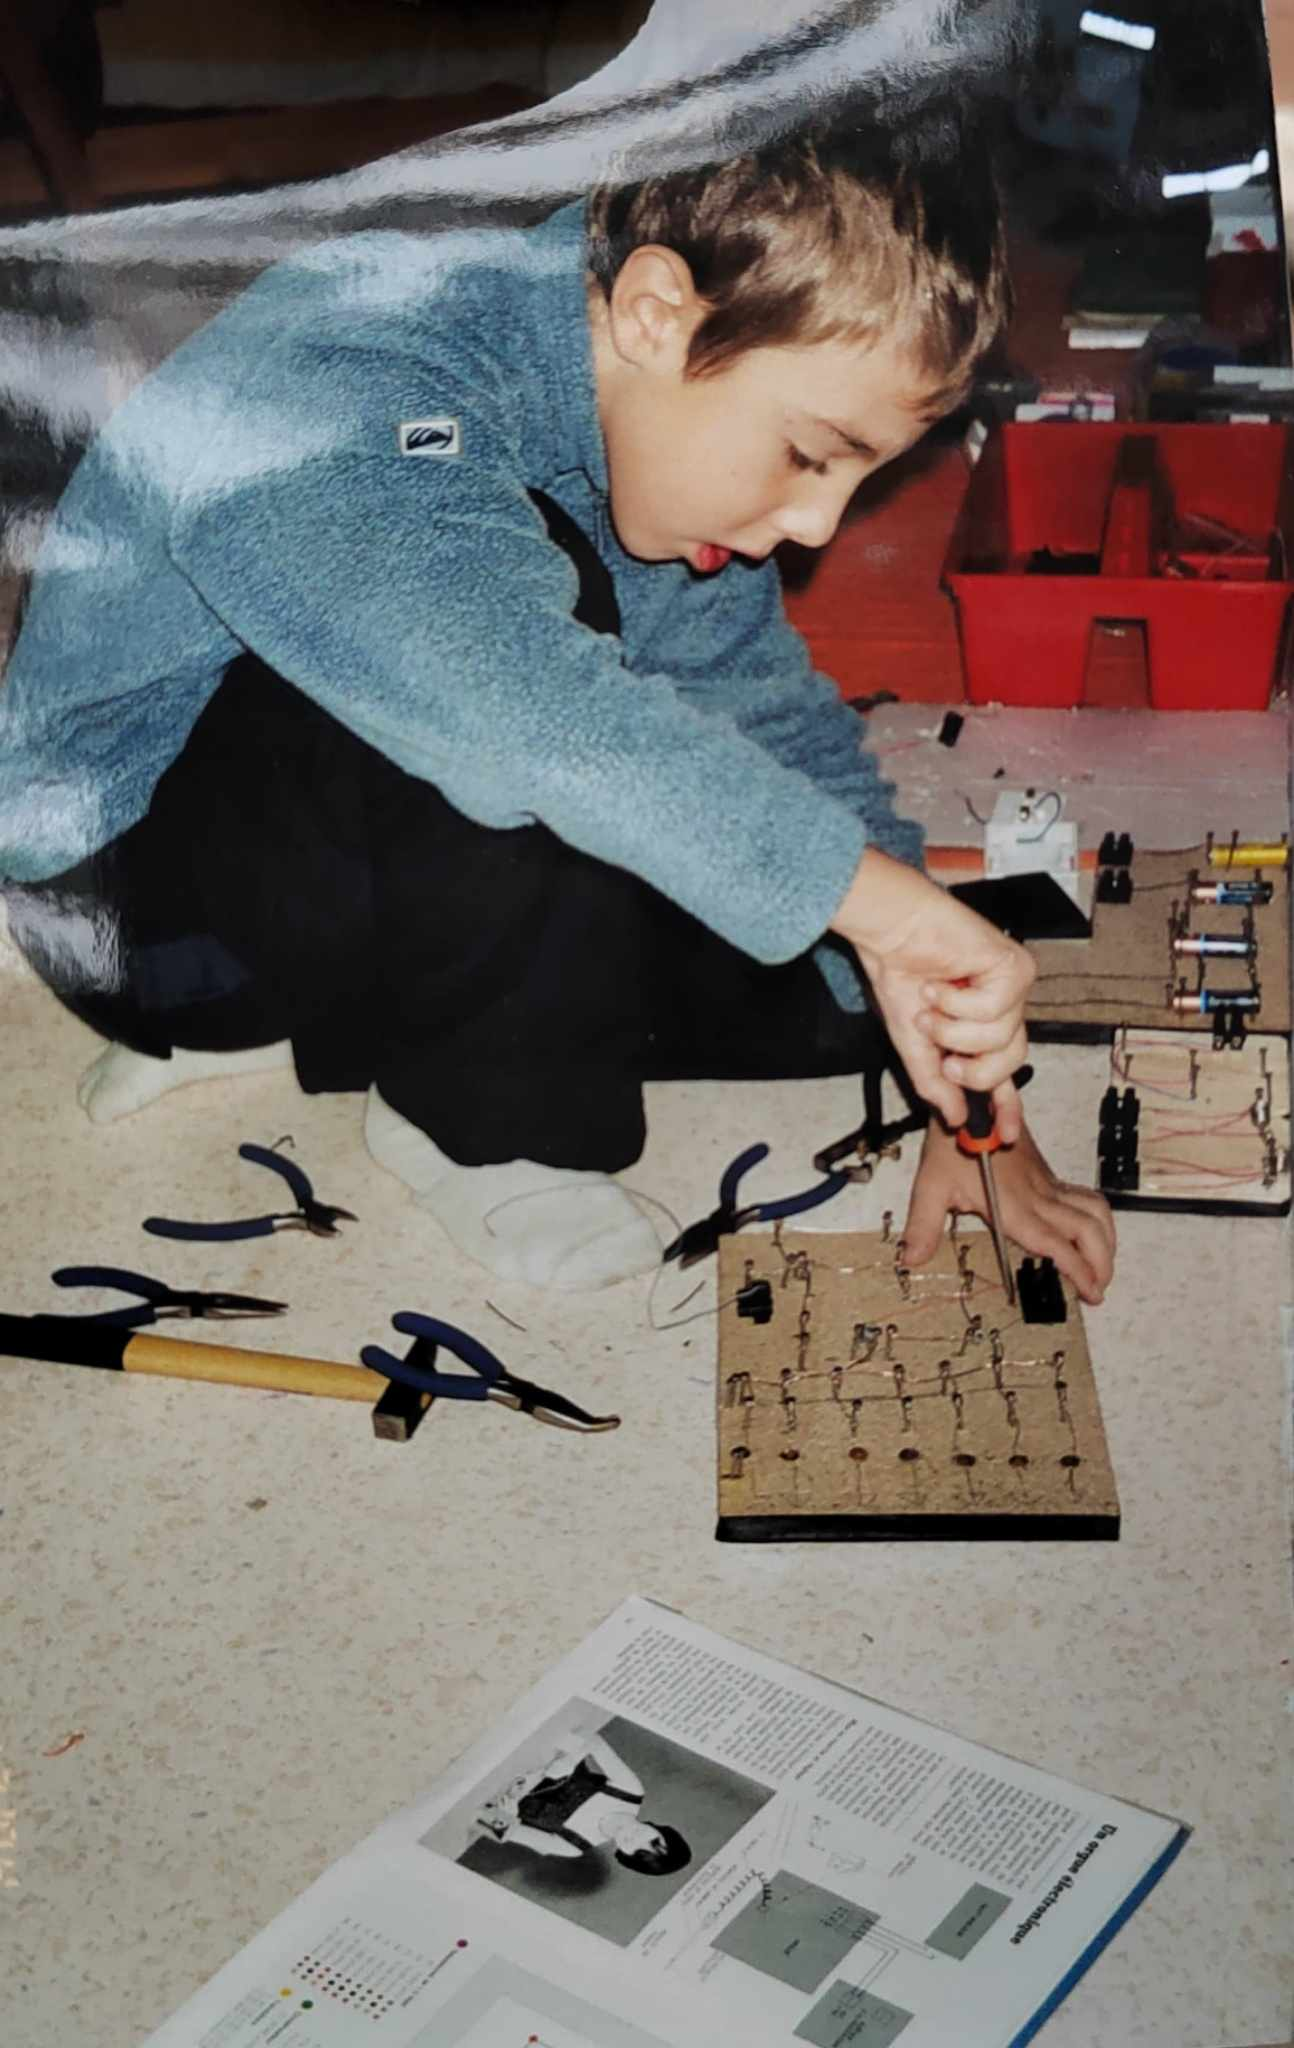
\includegraphics[width=0.85\textwidth]{moi2.jpg}
		%\caption{Proud of my weldings}
	\end{figure}
\end{column}
\end{columns}
\end{frame}

